\documentclass[letterpaper,spanish,12pt]{report} 
\usepackage[lmargin=2.3cm,
rmargin=2.3cm,top=2.5cm,bottom=2.5cm]{geometry}
\usepackage[spanish]{babel}
\usepackage{graphicx}
\usepackage{subfigure}
\usepackage{listings}
\begin{document}
%Portada%
\begin{titlepage}
\begin{center}
\vspace*{2cm}
\begin{figure}[htp]
\centering

\includegraphics[scale=0.3]{logo}
\end{figure}
\large{INSTITUTO TECN\'OLOGICO DE MORELIA\\ DEPARTAMENTO DE INGENIER\'IA ELECTR\'ONICA}
\rule{150mm}{0.1mm}\vspace{1.2cm} 
{\bf\Large CONTROL I}\\\vspace{0.8cm} {\bf{\huge Practica No. 2}\\ {\LARGE POLOS Y CEROS ENCONTRADOS POR INSPECCION}}\\\vspace{0.8cm} 
\begin{tabular*}{15cm}{l@{\extracolsep{\fill}}l}
{\Large Ariadne Paola Gonz\'alez Gallegos} & {\Large 13121114}\\
{\Large Jos\'e Abel Guti\'errez \'Alvarez} & {\Large 13121117}\\
\end{tabular*}
\vspace{0.8cm}\\\rule{150mm}{0.1mm}
\end{center}
\end{titlepage}
\tableofcontents \cleardoublepage
\addcontentsline{toc}{chapter}{Introducci\'on}
%Fin de la portada inicio del reporte%
\chapter*{Introducci\'on}
Con anterioridad ya vimos como es que para sistemas de primer orden una forma de obtener la funci\'on de transferencia es por medio de m\'etodos de an\'alisis electr\'onico tradicionales, y que en caso de tener un sistema distinto a este, como lo son hidr\'aulico o mec\'anico, siempre podemos realizar una analog\'ia entre ellos. La forma de hacerlo es simple, consiste en obtener las formulas de balance de energ\'ia que definen al sistema y luego despejar una variable de salida sobre una de entrada, de tal forma que el termino resultante sera la ecuaci\'on que defina el comportamiento de nuestro sistema. \\ Pero, �Qu\'e pasa si el sistema no es tan simple?, �Qu\'e pasa con un circuito mas complejo?, bueno, obtener la funci\'on de transferencia de este por m\'etodos tradicionales puede ser un proceso medianamente complicado o realmente complicado, dependiendo del sistema, y de nuestra capacidad para el \'algebra, pero existe una forma mas simple de hacerlo, este m\'etodo consiste en encontrar algunas variables de inter\'es del circuito, como su punto de DC, sus polos y sus ceros, de tal manera que al utilizar esta informaci\'on podamos encontrar la funci\'on de transferencia del circuito mucho mas f\'acil, este m\'etodo es c\'omodo ya que la expresi\'on que se obtiene ya esta simplificada y tiene una forma con la cual, con la misma informaci\'on, podemos encontrar la funci\'on de transferencia en circuitos de segundo orden. \\ En esta practica compararemos ese m\'etodo con el utilizado en la practica anterior, tambi\'en utilizaremos un entorno de simulaci\'on tipo SPICE para realizar una predicci\'on de las respuestas en el tiempo y la frecuencia, y luego obtendremos las reales, para ver si se cumple lo que esperamos o no.

%%%%%%%%%%%%%%%%%%%%%%%%%%%%%%%%%%%%%%%%%%%%%%%%%%%%%%%%%%%%%

	\renewcommand{\chaptername}{Parte}

	\chapter{Metodolog\'ia.}

	\section{Obteni\'endola por el M\'etodo de Polos y Ceros}

Para esta secci\'on vamos a utilizar la t\'ecnica de polos y ceros que aprendimos durante la parte te\'orica de la materia, con el fin de obtener la funci\'on de transferencia de el circuito mostrado en la figura \ref{cir:1} y de la figura \ref{cir:2}.\\ \medskip

\begin{figure}[h]
	\centering
		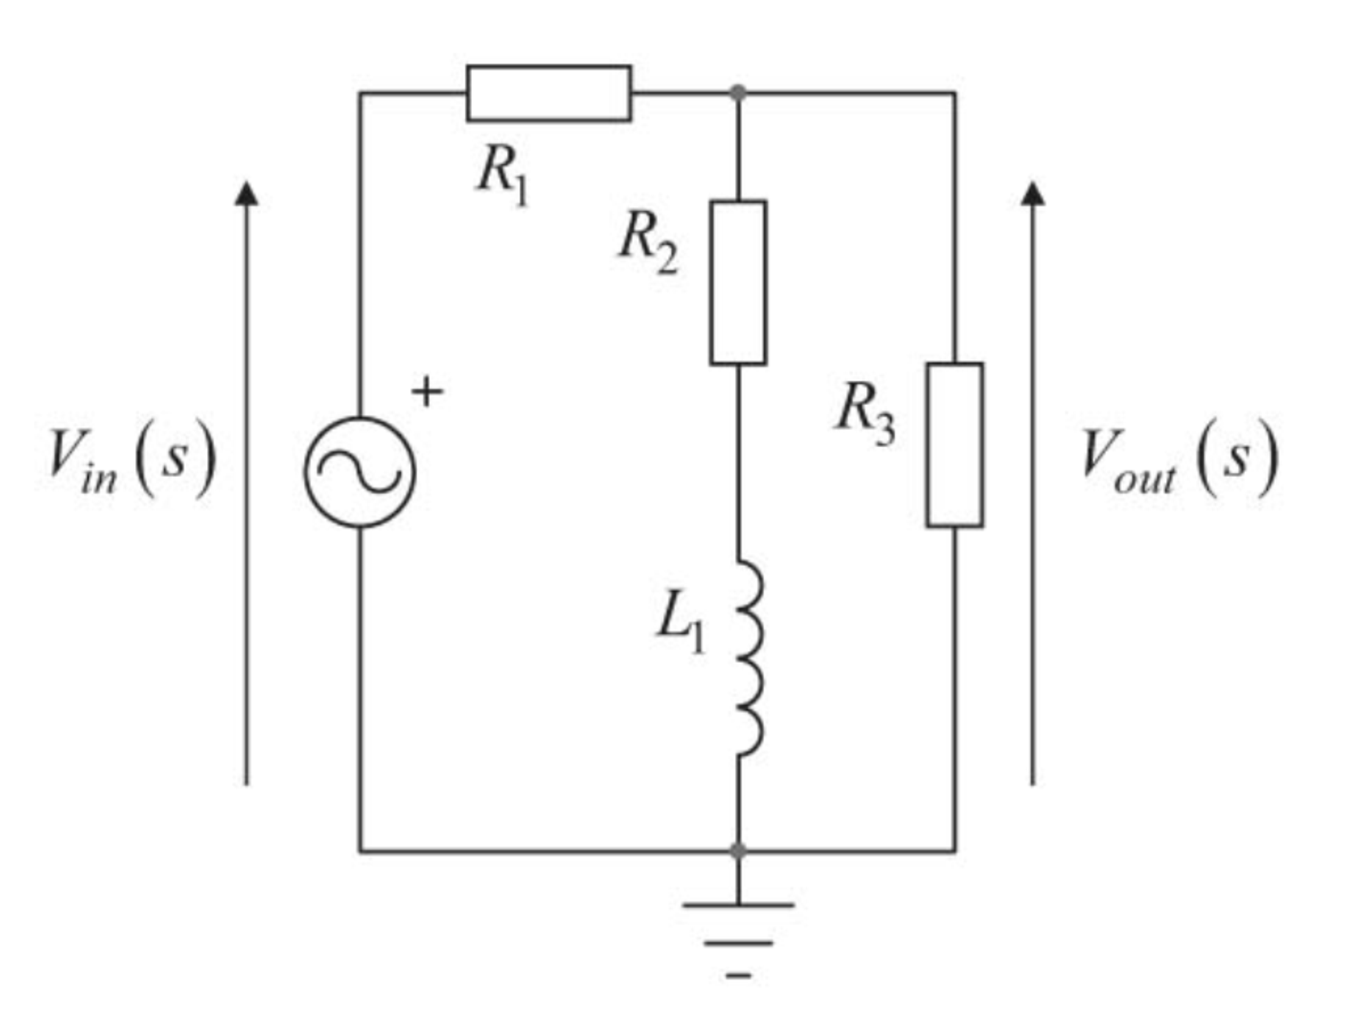
\includegraphics[width=0.50\textwidth]{Circuito1.eps}
	\caption{Circuito para la parte 1 con inductor}
	\label{cir:1}
\end{figure}

\begin{figure}[h]
	\centering
		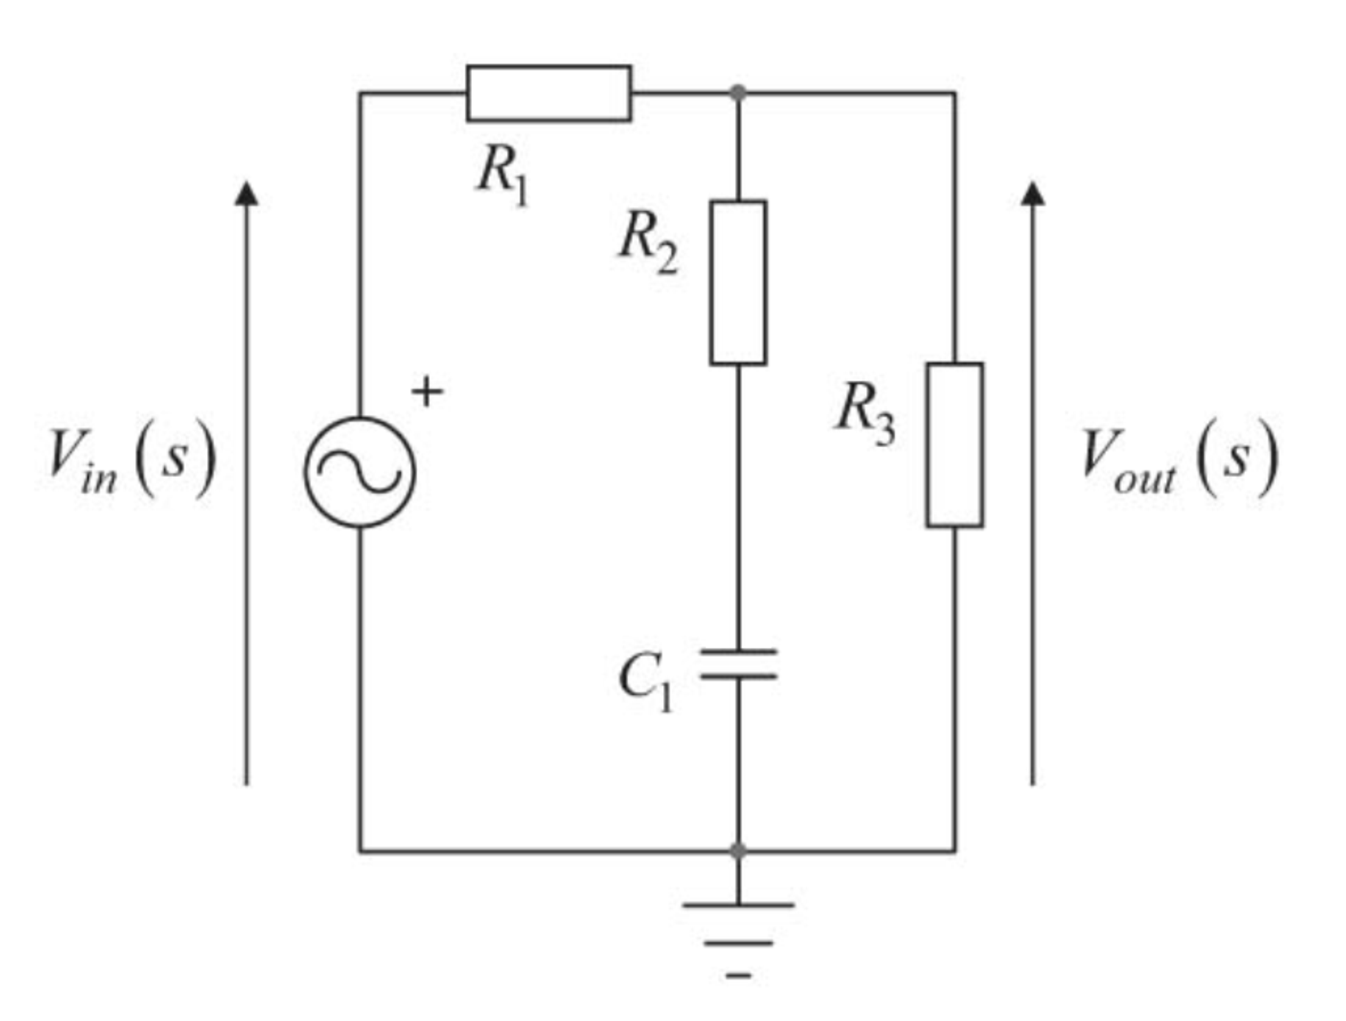
\includegraphics[width=0.50\textwidth]{Circuito4.eps}
	\caption{Circuito para la parte 1 con capacitor}
	\label{cir:2}
\end{figure}


Como podemos apreciar es un circuito de primer orden, solo que es un poco mas complejo que los vistos en la practica anterior. Ahora, para obtener la funci\'on de transferencia por medio de polos y ceros primero tenemos que definir que para este m\'etodo la funci\'on de transferencia estar\'a dada por la formula: \\ \medskip

	\begin{equation}
		\centering
		H(s) = \frac {V_{out}(S)} {V_{in}(S)} = G_{0} \frac {1 + \frac {S} {W_{z1}} } {1 + \frac {S} {W_{p1}} }  
		\label{ecu:1}
	\end{equation}

\medskip Ahora que sabemos esto debemos de encontrar los valores de $G_{0}$, $W_{z1}$ y $W_{p1}$. \medskip \\ La forma de encontrarlos es diferente para cada uno, iniciemos por $G_{0}$, cuyo valor se obtiene por medio del punto de operaci\'on de DC, en este caso se obtiene sustituyendo los inductores por un circuito cerrado, y los capacitores por un circuito abierto, obteniendo las figuras \ref{cir:3} y \ref{cir:5} respectivamente, y sus $G_{0}$ se obtienen midiendo el voltaje a la salida, es decir en $R3$, primero haremos todo el proceso para un inductor, y despu\'es para un capacitor. El circuito equivalente quedar\'ia como el de la figura \ref{cir:3}. \\ \medskip 

	\begin{figure}[h]
		\centering
			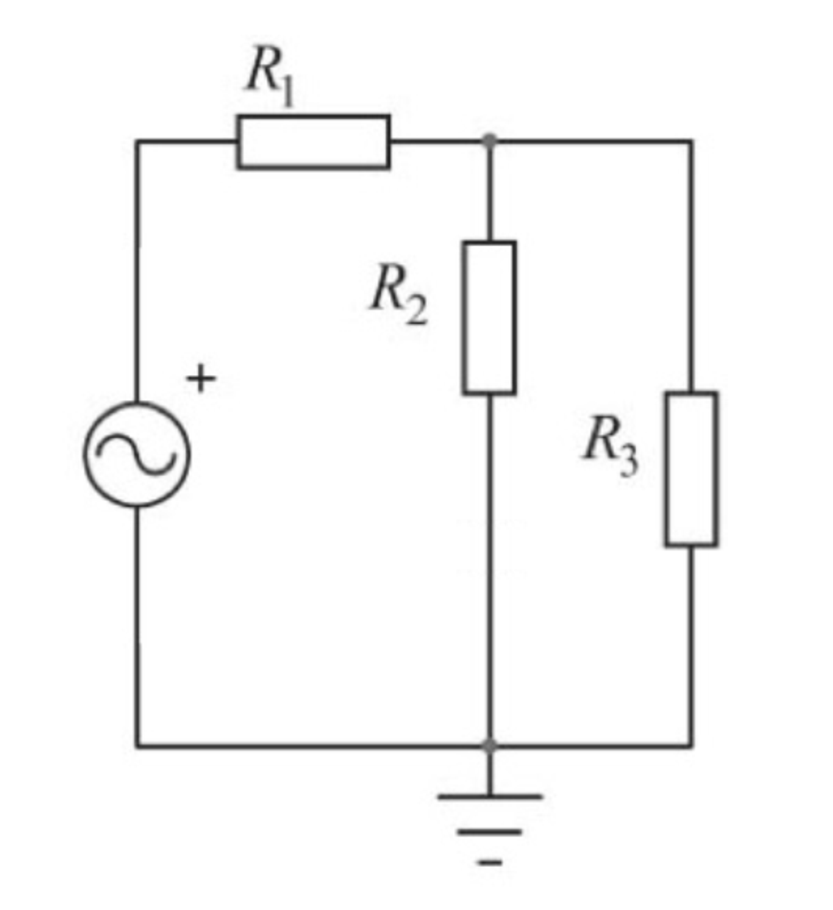
\includegraphics[width=0.50\textwidth]{Circuito2.eps}
		\caption{Circuito para obtener el DC point de un inductor}
		\label{cir:3}
	\end{figure}

Por lo tanto su $G_{0}$ seria: \\

	\begin{equation}
		\centering
		G_{0} = \frac { \frac {R_{2} R_{3}} {R_{2} + R_{3}} } {R_{1} + \frac {R_{2} R_{3}} {R_{2} + R_{3}} } =\frac { \frac {R_{2} R_{3}} {R_{2} + R_{3}} } {\frac {R_{1} R_{2} + R_{1} R_{3} + R_{2} R_{3} } {R_{2} + R_{3} } }  = \frac { R_{2} R_{3} } { R_{1} R_{2} +  R_{1} R_{3} + R_{2} R_{3} }
		\label{ecu:2}
	\end{equation}

Para calcular su $W_{z1}$ tendr\'iamos que encontrar la frecuencia donde el $V_{out} = 0$ para el circuito original con inductor, y en este caso el \'unico componente que afecta a la salida con respecto a la frecuencia es el inductor, y la rama que este afecta es en la que se encuentra en serie con $R_{2}$, y por casualidad el voltaje en $R_{3}$ es el mismo que en la rama de $R_{2}+SL_{1}$, e igualando este voltaje a cero y trabajando en el dominio de la frecuencia:

	\begin{center} $R_{2} + SL_{1} = 0$ \end{center}

Y haciendo un despeje para hacer quede de la forma:

	\begin{center} $1 + \frac {S} {W_{z1}} = 0 $ \end{center}

Obtenemos que:

	\begin{center} $1 + \frac {SL_{1}} {R_{2}} = 0 $ \end{center}

Y deducimos que:

	\begin{equation}
		\centering
		W_{z1} = \frac {R_{2}} {L_{1}} 
		\label{ecu:3}
	\end{equation}

Posteriormente pasaremos a calcular $W_{p1}$, para hacer esto primero necesitamos encontrar la resistencia vista desde las terminales del inductor o capacitor, esto se hace, como ya sabemos, por medio de la resistencia de Thevenin. Para el caso del inductor, el circuito que nos quedar\'ia como el de la figura \ref{cir:4}.

\begin{figure}[h]
	\centering
		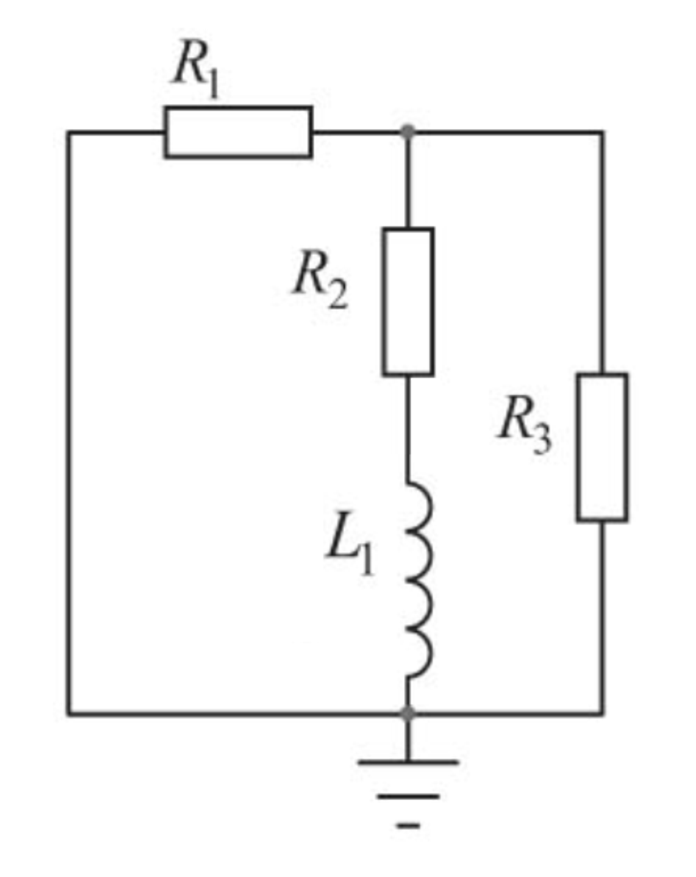
\includegraphics[width=0.50\textwidth]{Circuito5.eps}
	\caption{Circuito para encontrar la resistencia vista por el inductor}
	\label{cir:4}
\end{figure}

Y la resistencia equivalente seria:

	\begin{center} $R_{equ} = R_{2} + R_{1}||R_{3}$ \end{center}

Ahora, con base en esa resistencia debemos calcular el valor de $\frac{1}{\tau}$, y ese sera el valor de $W_{p1}$, sabiendo que $\tau = \frac {L} {R}$ deducimos que:

	\begin{equation}
		\centering
		W_{p1} = \frac{1}{\tau} = \frac{R}{L} = \frac{R_{2} + R_{1}||R_{3}}{L_{1}} = \frac{ R_{2}+\frac{R_{1}R_{3}}{R_{1}+R_{3}} }{L_{1}} = \frac{ (\frac{R_{1}R_{2}+R_{1}R_{3}+R_{2}R_{3}}{R_{1}+R_{3}}) }{(\frac{L_{1}}{1})} = \frac{R_{1}R_{2}+R_{1}R_{3}+R_{2}R_{3}}{L_{1}R_{1}+L_{1}R_{3}}
		\label{ecu:4}
	\end{equation}

Sustituyendo las ecuaciones \ref{ecu:2}, \ref{ecu:3} y la \ref{ecu:4} en la ecuaci\'on \ref{ecu:1}, y obtenemos:

	\begin{center} $H(S) = ( \frac{R_2||R_{3}}{R_{1}+R_2||R_{3}} ) (\frac{1+\frac{SL_{1}}{R_{2}}}{1+\frac{S(R_{2}+R_{1}||R_{3})}{L_{1}}})$ \end{center}

Para realizar un manejo mas simple de la funci\'on de transferencia del circuito, la llevaremos a su forma est\'andar utilizando \'algebra de la siguiente manera:

\begin{center}$H(S) = ( \frac{R_2||R_{3}}{R_{1}+R_2||R_{3}} ) (\frac{1+\frac{SL_{1}}{R_{2}}}{1+\frac{S(R_{2}+R_{1}||R_{3})}{L_{1}}})$\end{center}

\begin{center}$= (\frac{R_{2}R_{3}}{R_{1}R_{2}+R_{1}R_{3}+R_{2}R_{3}})(\frac{1+\frac{SL_{1}}{R_{2}}}{1+\frac{SL_{1}}{R_{2}+R_{1}||R_{3}}})$\end{center}

\begin{center}$= (\frac{R_{2}R_{3}}{R_{1}R_{2}+R_{1}R_{3}+R_{2}R_{3}})(\frac{\frac{R_{2}+SL_{1}}{R_{2}}}{1+\frac{(\frac{SL_{1}}{1})}{(\frac{R_{1}R_{2}+R_{1}R_{3}+R_{2}R_{3}}{R_{1}+R_{3}})}})$\end{center}

\begin{center}$= (\frac{R_{2}R_{3}}{R_{1}R_{2}+R_{1}R_{3}+R_{2}R_{3}})(\frac{\frac{R_{2}+SL_{1}}{R_{2}}}{1+\frac{SL_{1}R_{1}+SL_{1}R_{3}}{R_{1}R_{2}+R_{1}R_{3}+R_{2}R_{3}}})$\end{center}

\begin{center}$= (\frac{R_{2}R_{3}}{R_{1}R_{2}+R_{1}R_{3}+R_{2}R_{3}})(\frac{\frac{R_{2}+SL_{1}}{R_{2}}}{\frac{R_{1}R_{2}+R_{1}R_{3}+R_{2}R_{3}+SL_{1}R_{1}+SL_{1}R_{3}}{R_{1}R_{2}+R_{1}R_{3}+R_{2}R_{3}}})$\end{center}

\begin{center}$= \frac{(R_{2})(R_{3})(R_{2}+SL_{1})}{(R_{2})(R_{1}R_{2}+R_{1}R_{3}+R_{2}R_{3}+SL_{1}R_{1}SL_{1}R_{3})}$\end{center}

\begin{center}$= \frac{R_{3}R_{2}+SL_{1}R_{3}}{(SL_{1})(R_{1}+R_{3})+(R_{1}R_{2}+R_{1}R_{3}+R_{2}R_{3})}$\end{center}

Y haciendo un ultimo acomodo tenemos que la funci\'on de transferencia en su forma est\'andar para el circuito de la parte 1 con inductor es la mostrada en la ecuaci\'on \ref{ecu:5}.

	\begin{equation}
		\centering
		H(S) = \frac{\frac{SR_{3}}{(R_{1}+R_{3})} + \frac{R_{2}R_{3}}{L_{1}(R_{1}+R_{3})}} {S+(\frac{R_{1}R_{2}+R_{1}R_{3}+R_{2}R_{3}}{L_{1}(R_{1}+R_{3})})}
		\label{ecu:5}
	\end{equation}

Ahora, haremos lo mismo para el circuito \ref{cir:2}.

\begin{figure}[h]
	\centering
		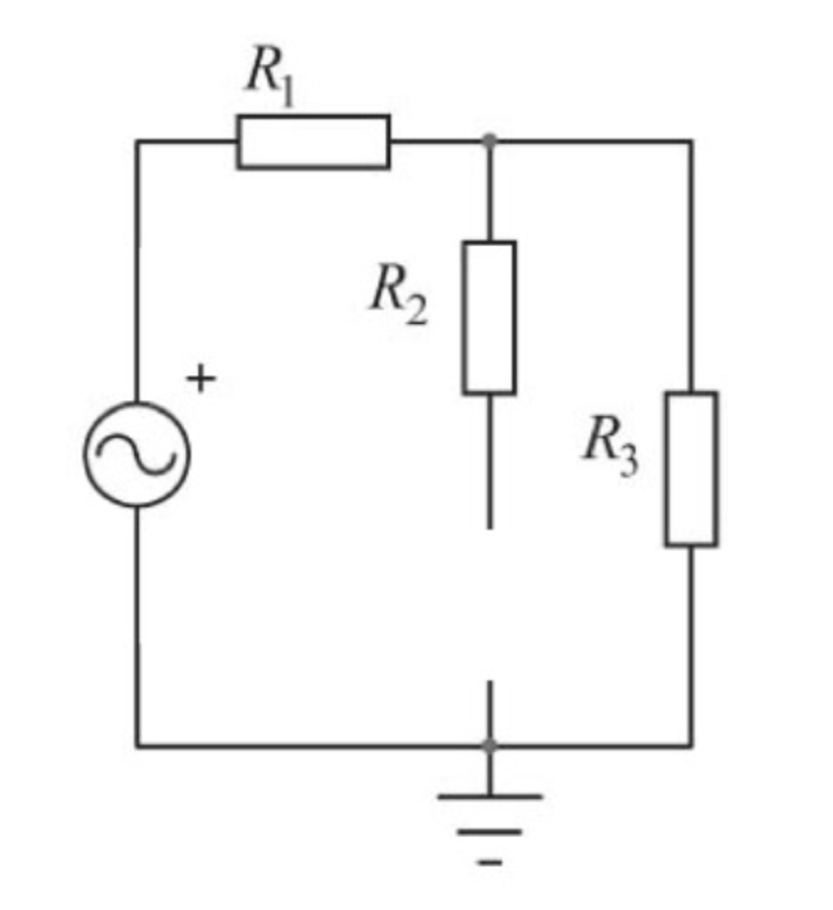
\includegraphics[width=0.50\textwidth]{Circuito3.eps}
	\caption{Circuito para obtener el DC point de un capacitor}
	\label{cir:5}
\end{figure}

Lo primero es obtener el termino $G_{0}$, y quedar\'ia como es mostrado en la ecuaci\'on \ref{ecu:6}.

	\begin{equation}
		\centering
		G_{0} = \frac { R_{3} } { R_{1} + R_{3} }
		\label{ecu:6}
	\end{equation}

Despu\'es debemos obtener el termino $W_{z1}$, al igual que en el caso del inductor, este valor sale de la rama de $R_{2}$ al igual que en el caso anterior y es el mostrado en la ecuaci\'on \ref{ecu:7}.

	\begin{equation}
		\centering
		W_{z1} = \frac{1}{C_{1}R_{2}}
		\label{ecu:7}
	\end{equation}

Y finalmente obtenemos $W_{p1}$, la $R_{equ}$ es la misma que en el caso del inductor, sin embargo la formula de $\tau$ es distinta, ya que en este caso su valor es $RC$, y por consecuencia el valor de $W_{p1}$ queda como en la ecuaci\'on \ref{ecu:8}.

	\begin{equation}
		\centering
		W_{p1} = \frac{R_{1}+R_{3}}{C_{1}(R_{1}R_{2}+R_{1}R_{3}+R_{2}R_{3})}
		\label{ecu:8}
	\end{equation}

Sustituyendo las ecuaciones \ref{ecu:6}, \ref{ecu:7} y \ref{ecu:8} en la ecuaci\'on \ref{ecu:1}, obtenemos la funcion de transferencia siguiente:

	\begin{center} $H(S) = (\frac{R_{3}}{R_{1}+R_{3}})(\frac{1+SC_{1}R_{2}}{1+(\frac{SC_{1}(R_{1}R_{2}+R_{1}R_{3}+R_{2}R_{3})}{R_{1}+R_{3}})})$ \end{center}

Pero aplicando \'algebra para pasar la funci\'on de transferencia en su forma est\'andar obtenemos la ecuaci\'on \ref{ecu:9}.

	\begin{equation}
		\centering
		H(S) = \frac{ S(\frac{R_{2}R_{3}}{R_{1}R_{2}+R_{1}R_{3}+R_{2}R_{3}}) + (\frac{R_{3}}{C_{1}(R_{1}R_{2}+R_{1}R_{3}+R_{2}R_{3})})}{ S + \frac{R_{1}+R_{3}}{C_{1}(R_{1}R_{2}+R_{1}R_{3}+R_{2}R_{3})} }
		\label{ecu:9}
	\end{equation}

	\section{Obteni\'endola la funci\'on de transferencia por m\'etodos tradicionales}

Ahora vamos a utilizar m\'etodos tradicionales para obtener la funci\'on de transferencia en la forma est\'andar de los circuitos \ref{cir:1} y \ref{cir:2}. \\ \medskip Para un inductor y utilizando el circuito \ref{cir:1} el proceso es el siguiente: \\ \medskip Primero establecemos las ecuaciones de mallas, para la malla 1 tenemos que:

	\begin{center}$V_{IN} = R_{1}I_{1}+R_{2}(I_{1}-I_{2})+SL_{1}(I_{1}-I_{2})$ \end{center}

Y para la malla 2:

	\begin{center}$R_{3}I_{2}+SL_{1}(I_{2}-I_{1})+R_{2}(I_{2}-I_{1}) = 0$ \end{center}

Ahora despejamos $I_{1}$ de la malla 1 y obtenemos que:

	\begin{center}$I_{1} = \frac{V_{IN}+I_{2}(R_{2}+SL_{1})}{R_{1}+R_{2}+SL_{1}}$ \end{center}

Y sustituimos este valor en la malla 2 de la siguiente forma:

	\begin{center}$I_{2}(R_{3}+SL_{1}+R_{2}) - (SL_{1}+R_{2})(\frac{V_{IN}+I_{2}(R_{2}+SL_{1})}{R_{1}+R_{2}+_{SL_{1}}})$\end{center}

De aqu\'i podemos despejar $I_{2}$ ya que esta es la corriente de salida ($I_{out}$), y con esta podemos obtener $V_{out}$ para finalmente tener la funci\'on de transferencia. As\'i que despejamos $I_{2}$:

	\begin{center}$I_{2}(R_{3}+SL_{1}+R_{2})(R_{1}+R_{2}+SL_{1}) - (SL_{1}+R_{2})(V_{IN}+I_{2}(R_{2}+SL_{1})) = 0$\end{center} 
	
	\begin{center}$I_{2}(R_{2}+R_{3}+SL_{1})(R_{1}+R_{2}+SL_{1}) - I_{2}(S^{2}L^{2}+2SL_{1}+R_{2}^{2}) = V_{IN}(SL_{1}+R_{2})$\end{center}

\begin{center}$I_{2}(R_{1}R_{2}+R_{1}R_{3}+R_{2}R_{3}+SL_{1}(R_{1}+R_{3})) = V_{IN}(SL_{1}+R_{2})$\end{center}

\begin{center}$\frac{I_{out}}{V_{IN}} = \frac{(SL_{1}+R_{2})(R_{3})}{SL_{1}(R_{1}+R_{3})+(R_{1}R_{2}+R_{1}R_{3}+R_{2}R_{3})}$\end{center}

Y para obtener $V_{out}$ se necesita multiplicar $I_{out}$ por $R_{3}$, as\'i que tenemos que:

\begin{center}$\frac{V_{out}}{V_{IN}} = \frac{SL_{1}R_{3}+R_{2}R_{3}}{SL_{1}(R_{1}+R_{3})+(R_{1}R_{2}+R_{1}R_{3}+R_{2}R_{3})}$\end{center}

Ya por ultimo solamente debemos de despejarla de forma que quede similar a:

\begin{center}$H(S) = \frac{bS + c}{S + a}$\end{center}

Y de esta manera finalmente llegamos a:

\begin{center}$H(S) = \frac{S(\frac{R_{3}}{R_{1}+R_{3}}) + \frac{R_{2}R_{3}}{L_{1}(R_{1}+R_{3})}}{S + \frac{R_{1}R_{2}+R_{1}R_{3}+R_{2}R_{3}}{L_{1}(R_{1}+R_{3})}}$\end{center}

Observando detenidamente la ecuaci\'on anterior podemos ver que es la misma que la ecuaci\'on que la \ref{ecu:5}, con esto se comprueba que ambas est�n correctas.

Ahora, para el capacitor es casi lo mismo, primero debemos obtener la malla 1:

	\begin{center}$V_{IN} = R_{1}I_{1}+R_{2}(I_{1}-I_{2})+(\frac{1}{SC_{1}})(I_{1}-I_{2})$\end{center}

Y la malla 2:

	\begin{center}$R_{3}I_{2}+(\frac{1}{SC_{1}})(I_{2}-I_{1})+R_{2}(I_{2}-I_{1}) = 0$ \end{center}

Como vemos las ecuaciones son las mismas que para el caso del inductor, sustituyendo $RL_{1}$ por $\frac{1}{RC_{1}}$ as\'i que omitiremos pasos hasta llegar a la parte donde se diferencia del anterior.

	\begin{center}$\frac{V_{out}}{V_{in}} = \frac{\frac{R_{3}}{SC_{1}} + (R_{2}R_{3})}{(\frac{R_{1}+R_{3}}{SC_{1}}) + (R_{1}R_{2}+R_{1}R_{3}+R_{2}R_{3})}$\end{center}

	\begin{center}$= \frac{\frac{1}{s}(\frac{R_{3}}{R_{1}+R_{3}}) + (\frac{C_{1}R_{2}R_{3}}{R_{1}+R_{3}})}{\frac{1}{s} + (\frac{C_{1}(R_{1}R_{2}+R_{1}R_{3}+R_{2}R_{3})}{R_{1}+R_{3}})}$\end{center}

	\begin{center}$= \frac{\frac{R_{3}(R_{1}+R_{3})+S(R_{1}+R_{3})(R_{2}R_{3})}{S(R_{1}+R_{3})(R_{1}+R_{3})}}{\frac{(R_{1}+R_{3})+SC_{1}(R_{1}R_{2}+R_{1}R_{3}+R_{2}R_{3})}{S(R_{1}+R_{3})}}$\end{center}
	
	\begin{center}$= \frac{R_{3}+SC_{1}R_{2}R_{3}}{(R_{1}+R_{3})+SC_{1}(R_{1}R_{2}+R_{1}R_{3}+R_{2}R_{3})}$\end{center}

	\begin{center}$= \frac{S(\frac{R_{2}R_{3}}{R_{1}R_{2}+R_{1}R_{3}+R_{2}R_{3}} + \frac{R_{3}}{C_{1}(R_{1}R_{2}+R_{1}R_{3}+R_{2}R_{3})})}{S + \frac{R_{1}+R_{3}}{C_{1}(R_{1}R_{2}+R_{1}R_{3}+R_{2}R_{3})}}$\end{center}

Y si comparamos esa ecuaci\'on con la ecuaci\'on \ref{ecu:9} vemos que son iguales, por lo cual comprobamos que ambas son correctas.

	\section{Comprobando en SciLab}

Ahora vamos a introducir las funciones \ref{ecu:5} y \ref{ecu:9} en el programa que generamos durante la practica pasada, con el fin de observar la respuesta de salida del circuito, el c\'odigo es:

\begin{verbatim}
function[y]=EcuGen(a,b,c)
tau = 1/a;
t = 0:tau/10:10*tau;
n=length(t);
u = c/a;
if a~=0 then
    for i=1:n
        y(1,i) = u + ((b-u)*exp(-a*t(i)));
    end
else
    for i=1:n
        y(n) = b;
    end
end
plot(t,y)
endfunction
\end{verbatim}

Y para tener datos exactos necesitamos conocer los valores de $R_{1}$, $R_{2}$, $R_{3}$, $L_{1}$ y $C_{1}$, los propondremos de valores que podamos implementar durante la parte f\'isica de la practica, as\'i que ser\'an de $100\Omega$ para las resistencias, $4.25mH$ para el inductor y $10\mu F$ para el capacitor.\\ \medskip Sabiendo esto podemos ingresar los valores en la funci\'on anterior y obtener las gr\'aficas de respuesta del circuito. Y estas quedan como las mostradas en la imagen \ref{cir:6} y \ref{cir:7}.

\begin{figure}[h]
	\centering
		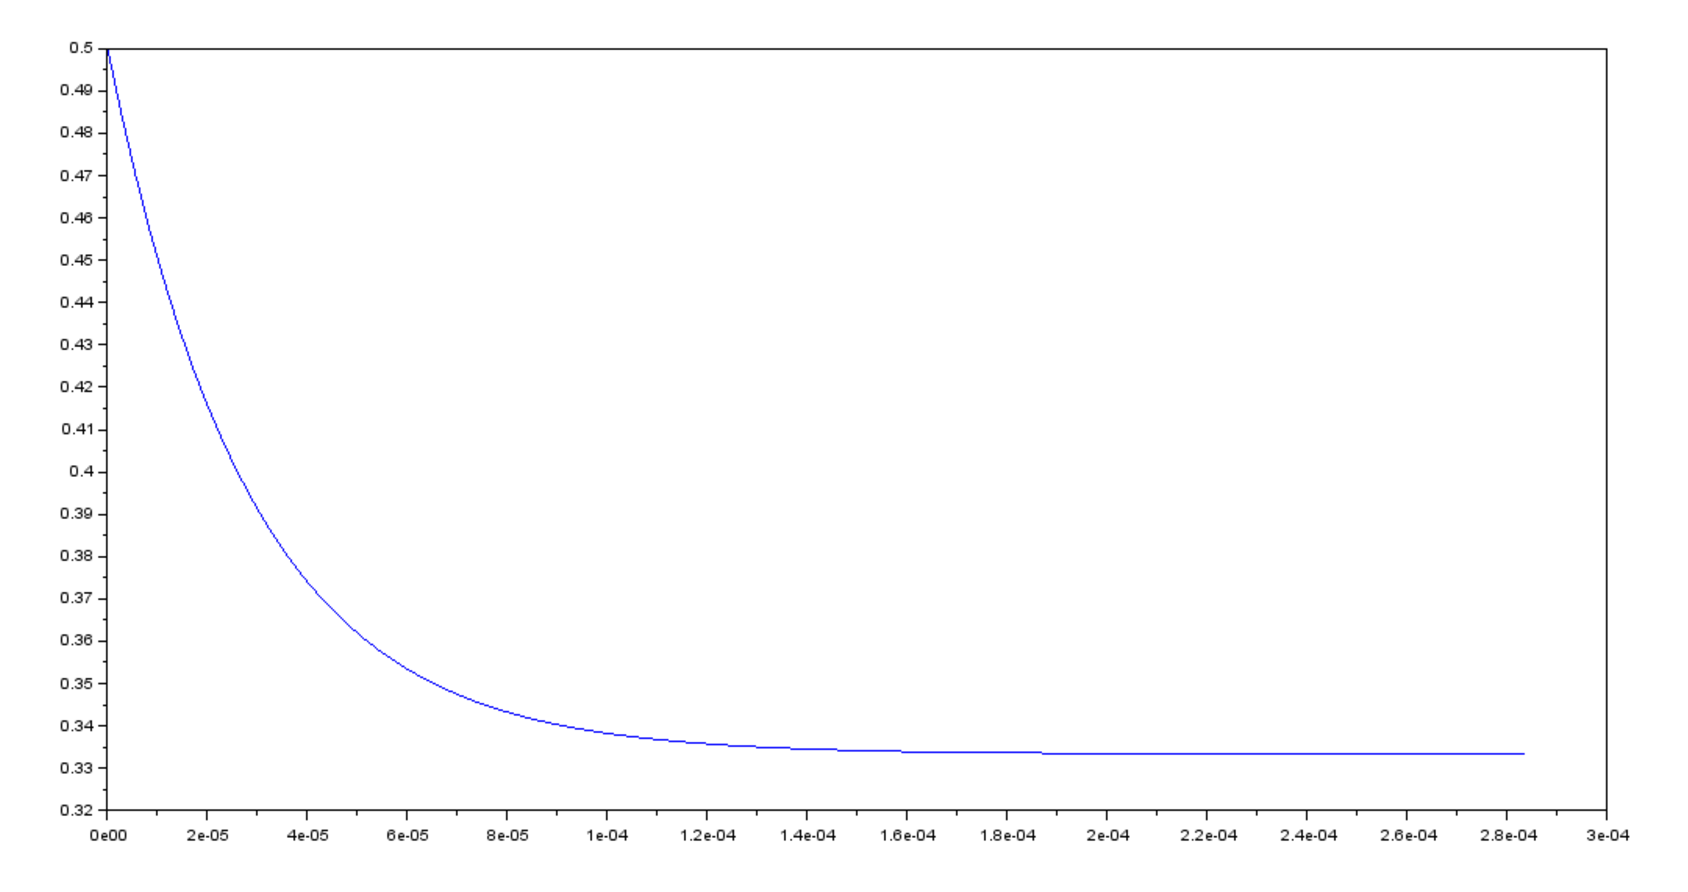
\includegraphics[width=1.00\textwidth]{FormadeondaL.eps}
	\caption{Respuesta de la funci\'on de transferencia para el circuito con inductor}
	\label{cir:6}
\end{figure}

\begin{figure}[h]
	\centering
		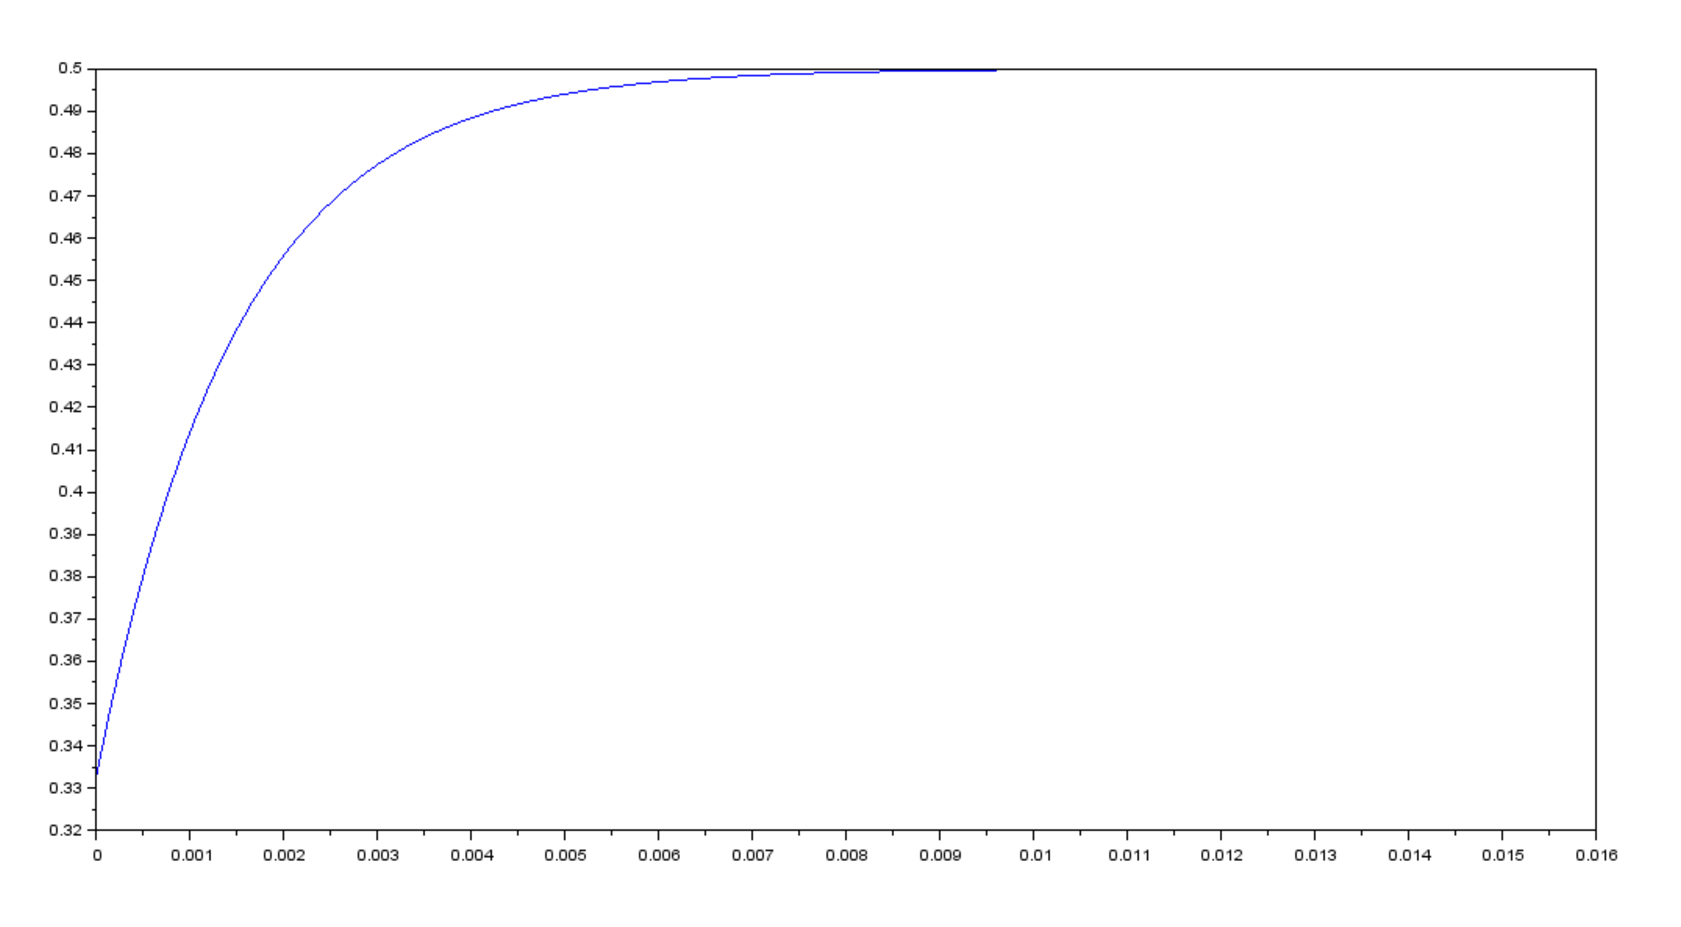
\includegraphics[width=1.00\textwidth]{FormadeondaC.eps}
	\caption{Respuesta de la funci\'on de transferencia para el circuito con capacitor}
	\label{cir:7}
\end{figure}

	\section{Obteniendo las formas de onda con LTI SPICE}

	\subsection{Respuesta en el tiempo}

En esta parte del reporte debemos de simular los circuitos de las figuras \ref{cir:1} y \ref{cir:2}, lo realizaremos en el entorno de simulaci\'on LTI SPICE, utilizaremos al igual que en el tercer inciso de la parte 1 los valores que usaremos de manera f\'isica en la parte 3 para simular, siendo $100\Omega$ para las resistencias $R_{1}$, $R_{2}$ y $R_{3}$, $4.25mH$ para el inductor y $10\mu F$ para el capacitor. \\ Y conociendo los valores podemos escribir el c\'odigo en SPICE para la respuesta de tiempo en el inductor:

\begin{verbatim}
Vin n1 GND PULSE(0v 5v 0s 10ns 10ns 7.5ms 15ms)
R1 n1 n2 100
R2 n2 n3 100
R3 n2 GND 100
L1 n3 GND 4.25mH
.TRAN 0.5us 50ms
\end{verbatim}

Y este genera la forma de onda mostrada en la figura \ref{cir:8}. \\ Ahora veamos la respuesta en el tiempo para el capacitor, y esta se genera con el siguiente c\'odigo:

\begin{verbatim}
Vin n1 GND PULSE(0v 5v 0s 10ns 10ns 7.5ms 15ms)
R1 n1 n2 100
R2 n2 n3 100
R3 n2 GND 100
C1 n3 GND 10uF
.TRAN 0.5us 50ms
\end{verbatim}

Y este genera la respuesta mostrada en la figura \ref{cir:9}.

\begin{figure}[h]
	\centering
		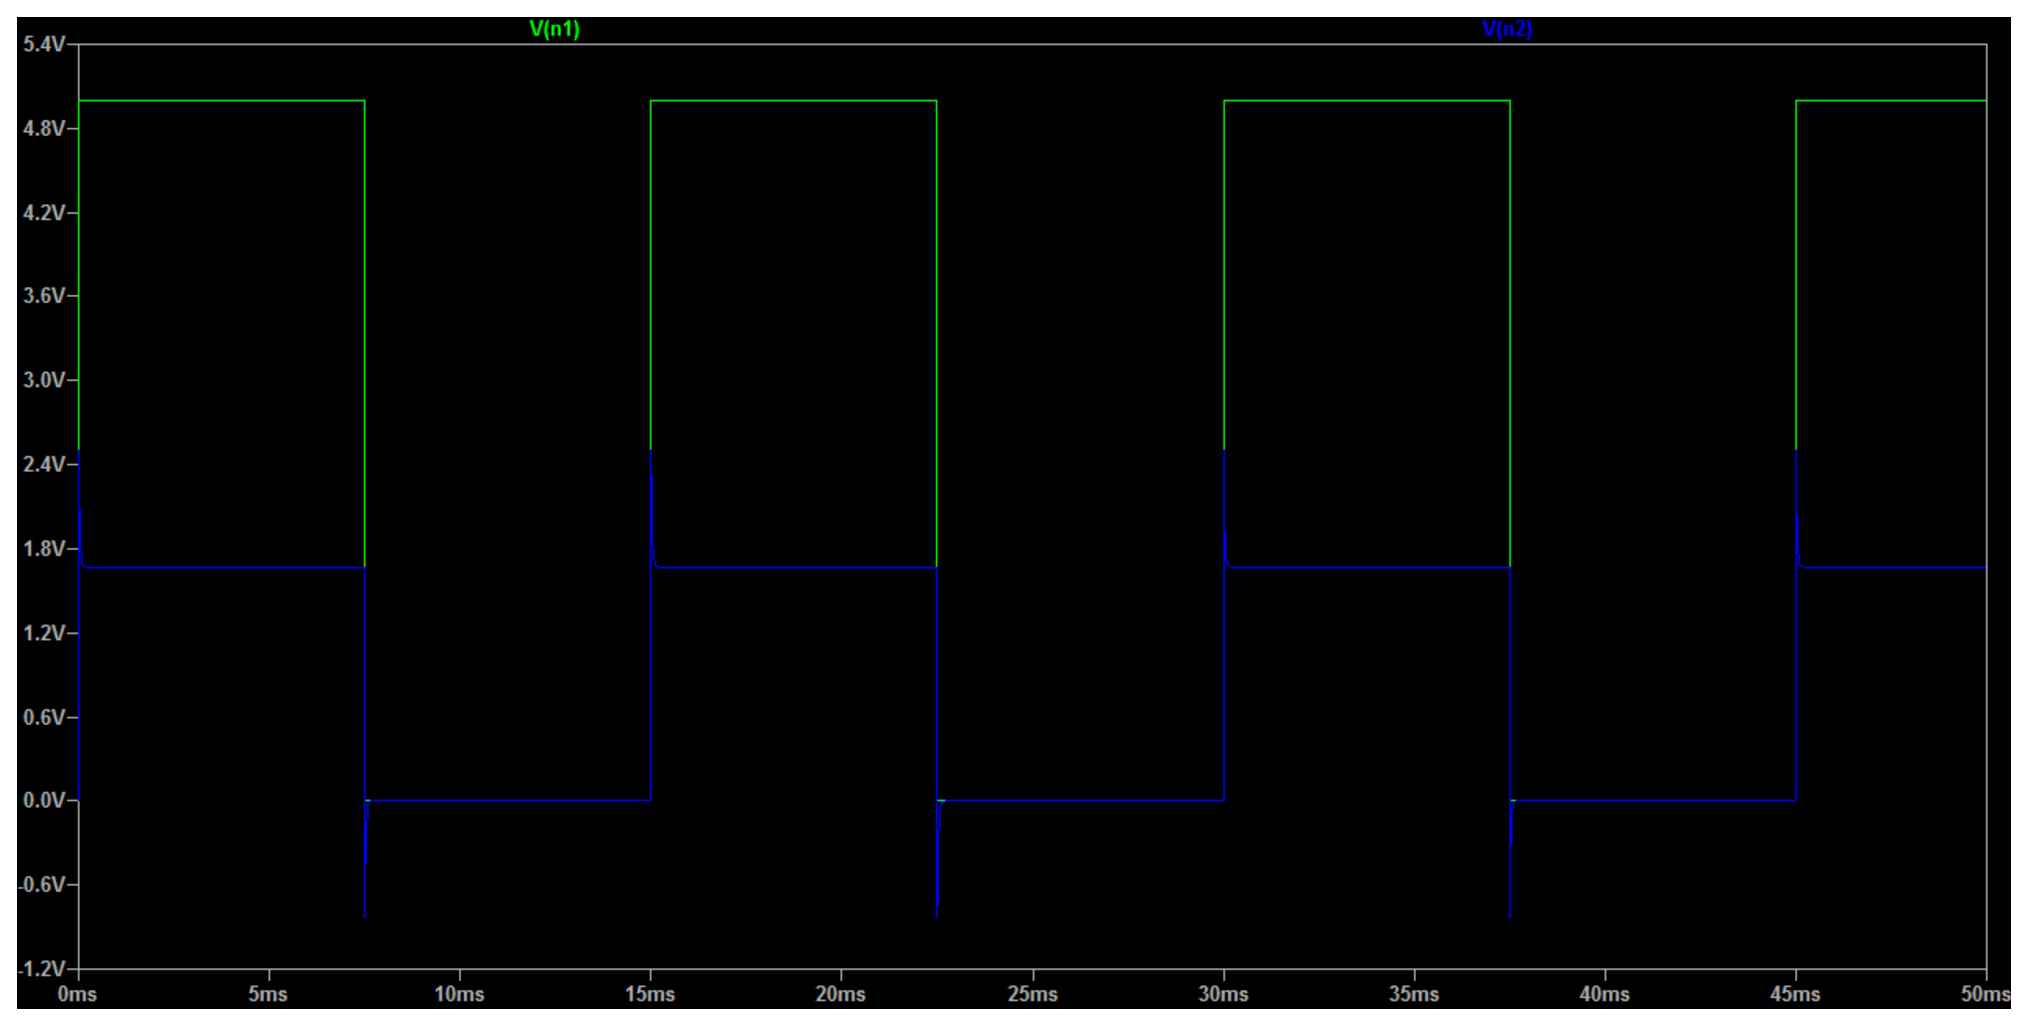
\includegraphics[width=0.80\textwidth]{ResTieL.eps}
	\caption{Respuesta en el tiempo para el inductor}
	\label{cir:8}
\end{figure}

\begin{figure}[h]
	\centering
		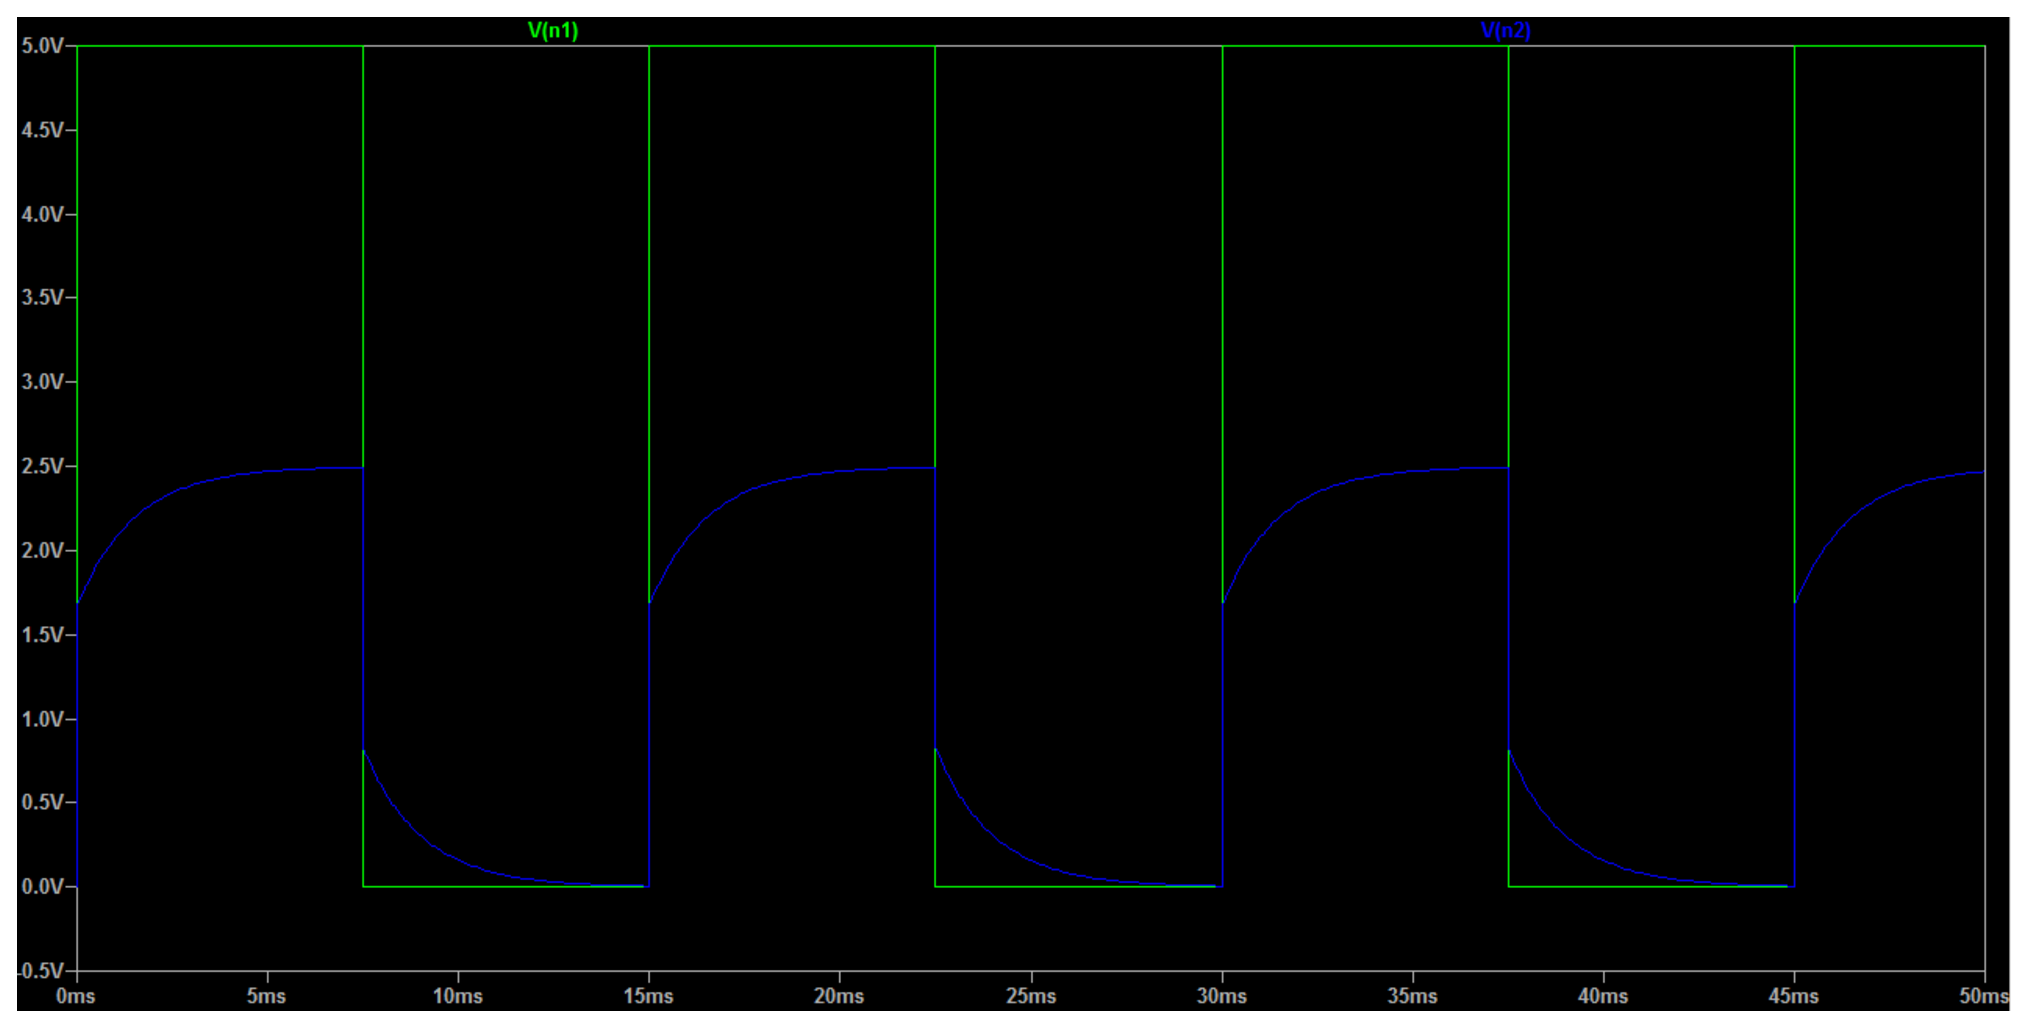
\includegraphics[width=0.80\textwidth]{ResTieC.eps}
	\caption{Respuesta en el tiempo para el capacitor}
	\label{cir:9}
\end{figure}

	\subsection{Respuesta en la frecuencia}

Ahora vamos con la respuesta en frecuencia, para el inductor esta dada por:

\begin{verbatim}
Vin n1 GND AC(2.5v)
R1 n1 n2 100
R2 n2 n3 100
R3 n2 GND 100
L1 n3 GND 4.25mH
.ac dec 10 100Hz 100kHz
\end{verbatim}

Y la respuesta que nos da es la mostrada en la figura \ref{cir:10}. \\ Mientras que para el capacitor, el c\'odigo es:

\begin{verbatim}
Vin n1 GND ac(2.5v)
R1 n1 n2 100
R2 n2 n3 100
R3 n2 GND 100
C1 n3 GND 10uF
.ac dec 10 1Hz 10kHz
\end{verbatim}

Y la respuesta en frecuencia del mismo es la mostrada en la figura \ref{cir:11}.

\begin{figure}[h]
	\centering
		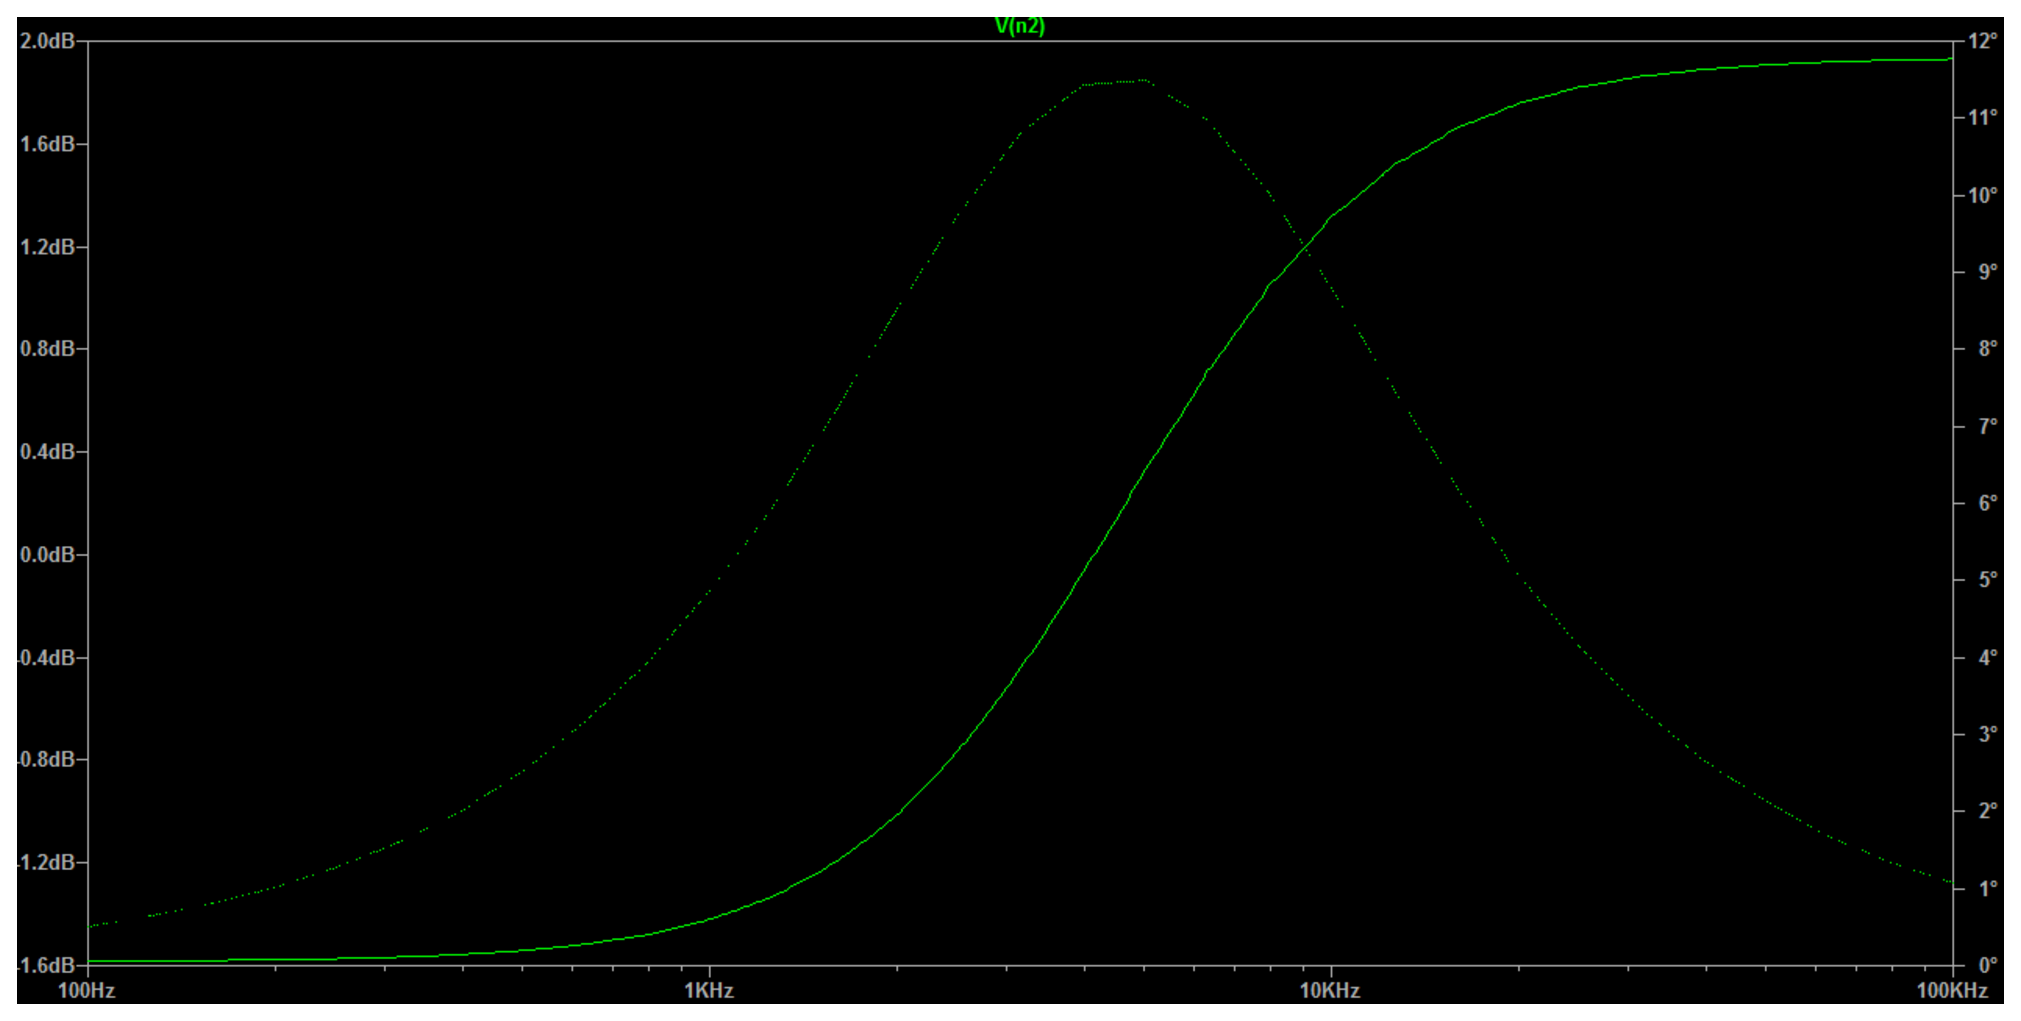
\includegraphics[width=0.80\textwidth]{ResFreL.eps}
	\caption{Respuesta en la frecuencia para el inductor}
	\label{cir:10}
\end{figure}

\begin{figure}[h]
	\centering
		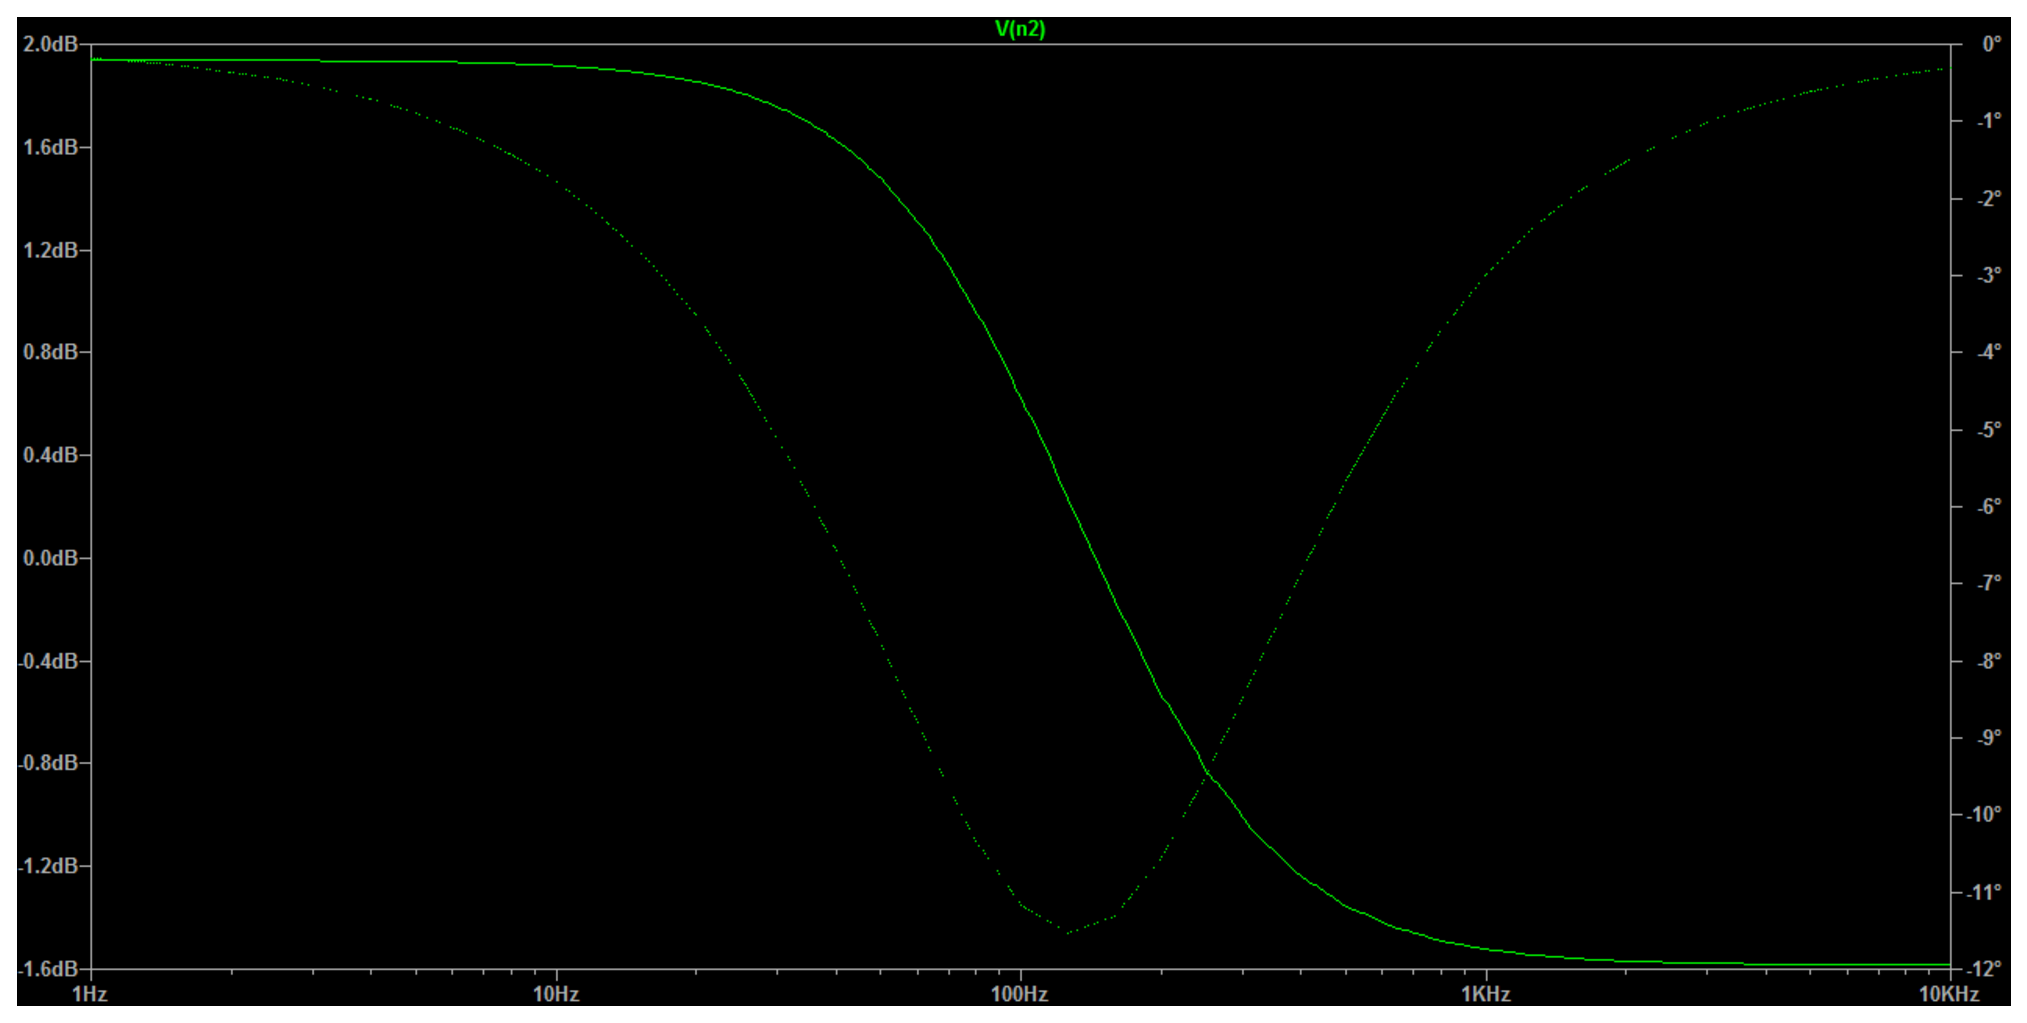
\includegraphics[width=0.80\textwidth]{ResFreC.eps}
	\caption{Respuesta en la frecuencia para un capacitor}
	\label{cir:11}
\end{figure}

	\chapter{Resultados y Discusi\'on}
	\section{Resultados y an\'alisis del circuito f\'isico}
	\subsection{Respuesta en el tiempo}

Para esta parte del reporte realizamos el circuito de manera f\'isica en el laboratorio, utilizamos los valores de resistencias en $100\Omega$, para el inductor de $4.25mH$ y para el capacitor de $10\mu F$, lo primero que se nos requiere es la forma de la respuesta en el tiempo, esta podemos medirla directamente en el osciloscopio, simplemente medimos la onda de entrada y la forma de onda en $R_{3}$. \\ \medskip Y obtuvimos la respuesta mostrada en la figura \ref{cir:12}.

\begin{figure}[h]
	\centering
		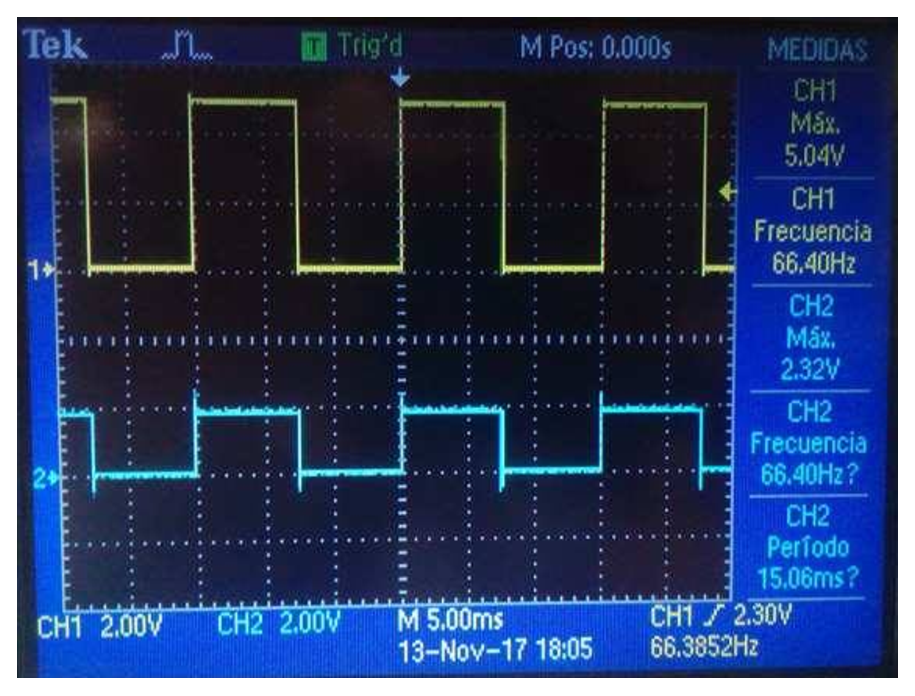
\includegraphics[width=0.50\textwidth]{ResReaTieL.eps}
	\caption{Respuesta real en el tiempo para el inductor}
	\label{cir:12}
\end{figure}

Y para el capacitor se hizo exactamente lo mismo, y obtuvimos las formas de onda mostradas en la figura \ref{cir:13}.

\begin{figure}[h]
	\centering
		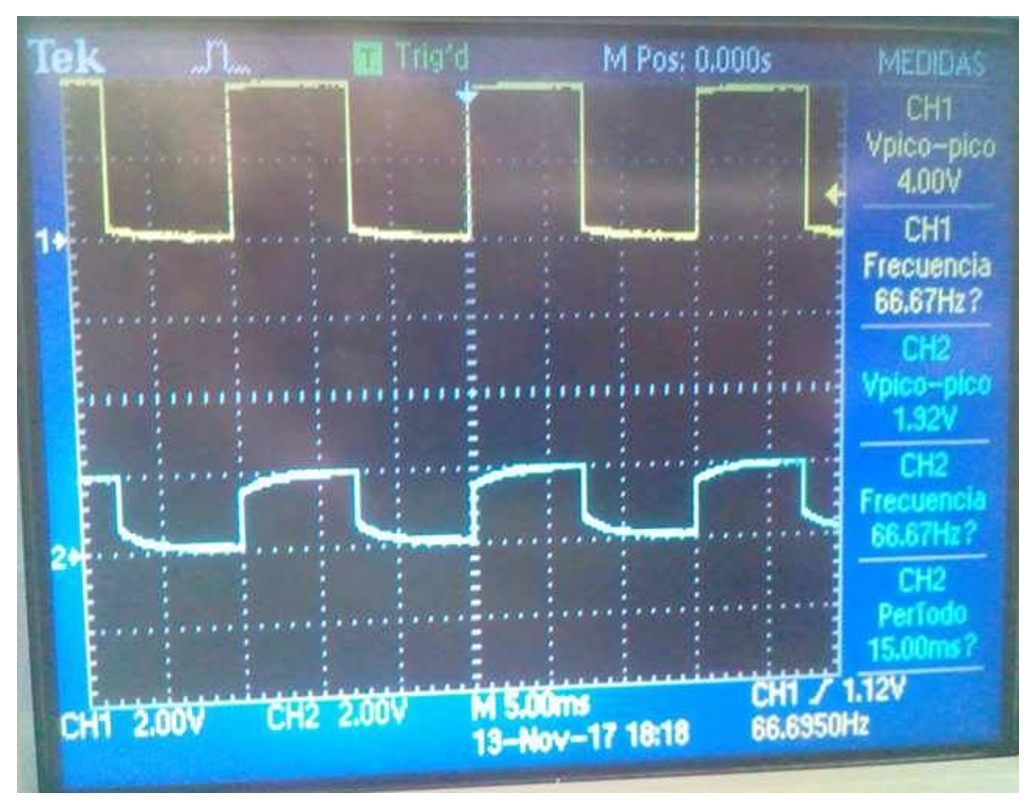
\includegraphics[width=0.50\textwidth]{ResReaTieC.eps}
	\caption{Respuesta real en el tiempo para el capacitor}
	\label{cir:13}
\end{figure}

	\subsection{Respuesta en la frecuencia}

Para esta parte no podemos solo realizar la medici\'on directa, no contamos con el equipo para realizar lo, as\'i que lo que hicimos fue alimentar el circuito con frecuencias distintas, diez frecuencias por cada d\'ecada, y capturamos las formas de onda, esto con el fin de mas tarde utilizando los valores de frecuencia y voltaje en la salida de cada captura, obtener la forma de la respuesta en frecuencia del circuito, y con la forma de onda de entrada, obtener la forma de la funci\'on de transferencia, esto con el fin de compararlas mas adelante en el reporte con las obtenidas en las partes previas.\\ Iniciemos generando una tabla con los valores para el inductor, esta queda como la de la tabla \ref{tab:1}.\\

% \multicolumn{numero de columnas}{lo que va en la columna}
% \multirow{numero de filas}{lo que va en la fila}
% & (para separar columnas)
% \hline (para separar filas con una linea)
% \\ (brincar a la siguiente linea)
% \cline{filas en las que escribiremos}

\begin{table}[h]
	\centering
		\begin{tabular}{|l|l|l|l|}
			\hline
			Numero de medici\'on & Frecuencia & Voltaje de entrada & 			Voltaje de salida\\
			\hline \hline
			1 & 100.8Hz & 3.8V & 1.56V \\
			\hline
			2 & 199.7Hz & 3.8V & 1.56V \\
			\hline
			3 & 299.4Hz & 3.8V & 1.56V \\
			\hline
			4 & 398.1Hz & 3.84V & 1.56V \\
			\hline
			5 & 505.1Hz & 3.84V & 1.64V \\
			\hline
			6 & 599.5Hz & 3.84V & 1.56V \\
			\hline
			7 & 701.3Hz & 3.88V & 1.64V \\
			\hline
			8 & 803.9Hz & 3.84V & 1.56V \\
			\hline
			9 & 897.7Hz & 3.84V & 1.6V \\
			\hline
			10 & 1.02kHz & 3.88V & 1.72V \\
			\hline
			11 & 2.002kHz & 3.92V & 1.76V \\
			\hline
			12 & 2.952kHz & 3.96V & 1.8V \\
			\hline
			13 & 4.082kHz & 3.96V & 1.8V \\
			\hline
			14 & 5.071kHz & 3.96V & 1.84V \\
			\hline
			15 & 5.97kHz & 3.96V & 1.92V \\
			\hline
			16 & 7.092kHz & 4.0V & 1.96V \\
			\hline
			17 & 8.188kHz & 4.0V & 1.96V \\
			\hline
			18 & 9.091kHz & 4.0V & 2.0V \\
			\hline
			19 & 10.01kHz & 4.04V & 2.04V \\
			\hline
			20 & 20.59kHz & 4.04V & 2.08V \\
			\hline
			21 & 31.0kHz & 4.08V & 2.16V \\
			\hline
			22 & 39.28kHz & 4.08V & 2.28V \\
			\hline
			23 & 50.15kHz & 4.08V & 2.4V \\
			\hline
			24 & 60.98kHz & 4.08V & 2.4V \\
			\hline
			25 & 69.96kHz & 4.08V & 2.32V \\
			\hline
			26 & 81.04kHz & 4.08V & 2.32V \\
			\hline
			27 & 89.93kHz & 4.16V & 2.4V \\
			\hline
			28 & 99.8kHz & 4.08V & 2.4V \\
			\hline
		\end{tabular}
	\caption{Datos del barrido en frecuencia}
	\label{tab:1}
\end{table}

Y para el capacitor tendr\'iamos los valores mostrados en la tabla \ref{tab:2}.

\begin{table}[h]
	\centering
		\begin{tabular}{|l|l|l|l|}
			\hline
			Numero de medici\'on & Frecuencia & Voltaje de entrada & 			Voltaje de salida\\
			\hline \hline
			1 & 3.09Hz & 4.16V & 1.76V \\
			\hline
			2 & 4.16Hz & 4.24V & 1.88V \\
			\hline
			3 & 5.0Hz & 4.24V & 1.96V \\
			\hline
			4 & 5.96Hz & 4.24V & 1.96V \\
			\hline
			5 & 7.02Hz & 4.24V & 2.0V \\
			\hline
			6 & 8.0Hz & 4.24V & 2.08V \\
			\hline
			7 & 9.02Hz & 4.24V & 2.08V \\
			\hline
			8 & 10.0Hz & 4.24V & 2.08V \\
			\hline
			9 & 19.97Hz & 4.16V & 2.08V \\
			\hline
			10 & 30.18Hz & 4.16V & 2.04V \\
			\hline
			11 & 40.29Hz & 4.08V & 2.0V \\
			\hline
			12 & 50.23Hz & 4.08V & 2.0V \\
			\hline
			13 & 60.19Hz & 4.08V & 1.92V \\
			\hline
			14 & 70.13Hz & 4.08V & 1.92V \\
			\hline
			15 & 80.28Hz & 4.08V & 1.88V \\
			\hline
			16 & 89.41Hz & 4.08V & 1.84V \\
			\hline
			17 & 100.54Hz & 4.08V & 1.8V \\
			\hline
			18 & 202.72Hz & 4.0V & 1.68V \\
			\hline
			19 & 301.66Hz & 3.92V & 1.56V \\
			\hline
			20 & 398.22Hz & 3.92V & 1.56V \\
			\hline
			21 & 507.1Hz & 3.92V & 1.52V \\
			\hline
			22 & 596.21Hz & 3.92V & 1.48V \\
			\hline
			23 & 696.5Hz & 3.92V & 1.48V \\
			\hline
			24 & 808.28Hz & 3.92V & 1.48V \\
			\hline
			25 & 899.6Hz & 3.92V & 1.48V \\
			\hline
			26 & 1.01kHz & 3.92V & 1.48V \\
			\hline
			27 & 2.02kHz & 3.92V & 1.48V \\
			\hline
			28 & 3.06kHz & 3.84V & 1.44V \\
			\hline
			29 & 4.06kHz & 3.92V & 1.44V \\
			\hline
			30 & 5.02kHz & 3.84V & 1.4V \\
			\hline
			31 & 6.01kHz & 3.84V & 1.4V \\
			\hline
			32 & 7.23kHz & 3.84V & 1.4V \\
			\hline
			33 & 8.06kHz & 3.84V & 1.4V \\
			\hline
			34 & 8.99kHz & 3.91V & 1.4V \\
			\hline
			35 & 10.06kHz & 3.84V & 1.4V \\
			\hline
		\end{tabular}
	\caption{Datos de barrido para el capacitor}
	\label{tab:2}
\end{table}

	\section{Graficando la respuesta en frecuencia}

Con los datos obtenidos en el paso anterior, podemos generar las formas de onda de la respuesta en frecuencia para el capacitor (figura \ref{cir:14}) y el inductor (figura \ref{cir:15}), y quedan como se muestra en sus respectivas im\'agenes.

\begin{figure}[h]
	\centering
		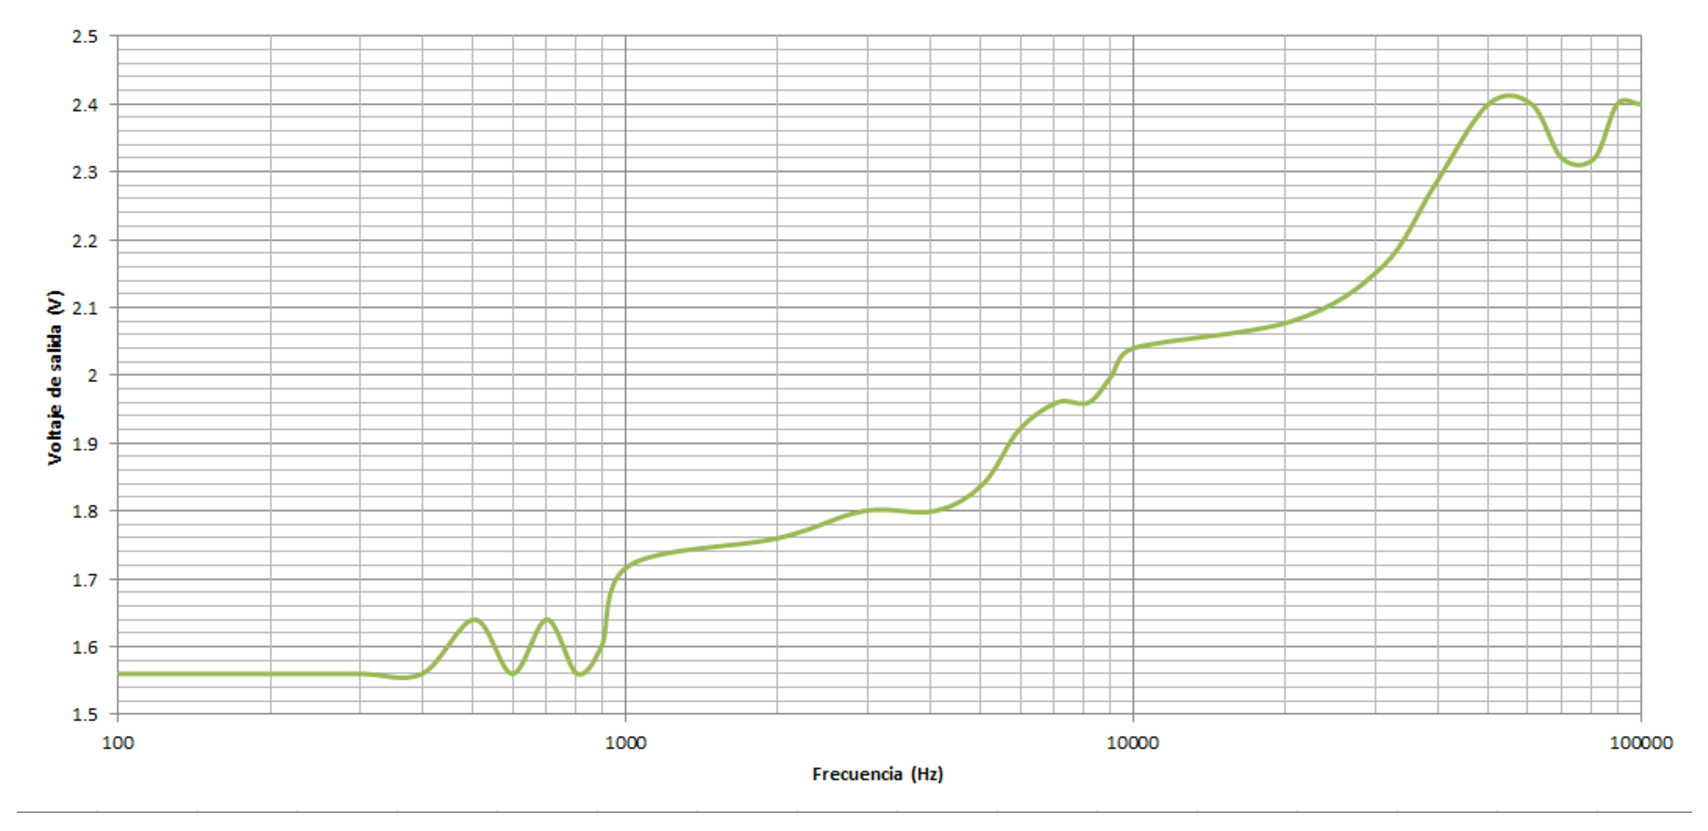
\includegraphics[width=1.00\textwidth]{ResReaFreL.eps}
	\caption{Respuesta real en la frecuencia para el inductor}
	\label{cir:14}
\end{figure}

\begin{figure}[h]
	\centering
		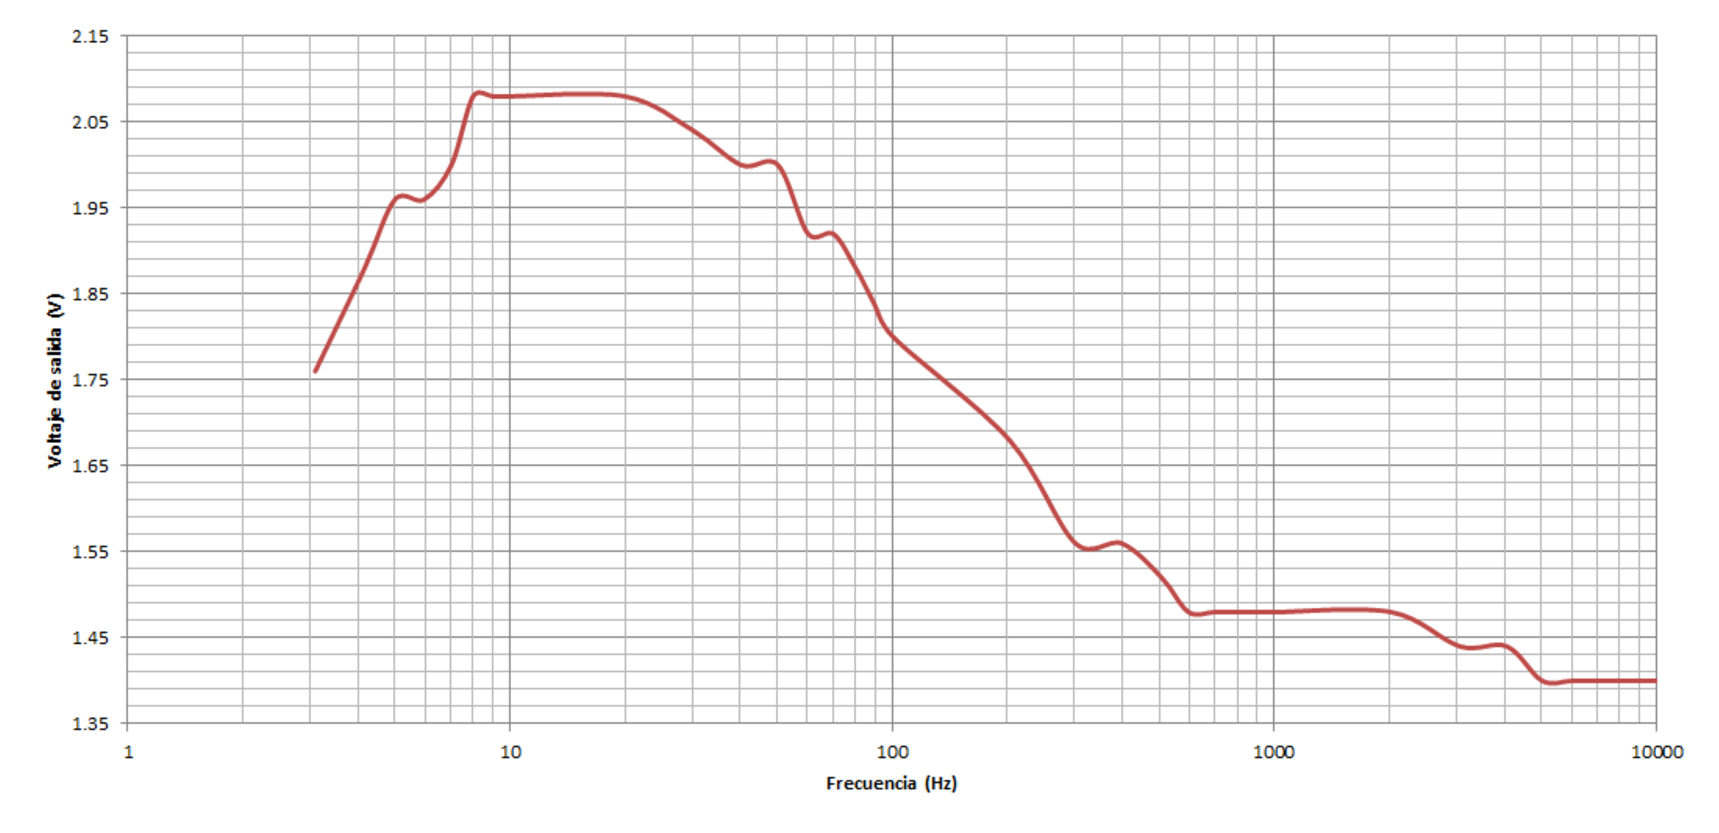
\includegraphics[width=1.00\textwidth]{ResReaFreC.eps}
	\caption{Respuesta real en la frecuencia para el capacitor}
	\label{cir:15}
\end{figure}

Ademas, agregando el voltaje de entrada real en el circuito podemos definir la funci\'on de transferencia con la formula $F.T(S) = \frac{V_{out}}{V_{in}}$, y con el inverso de la frecuencia obtenemos el periodo, d\'andonos la oportunidad de graficar la funci\'on de transferencia para el circuito con el inductor y con el capacitor, las cuales quedar\'ia como se muestra en las figuras \ref{cir:16} y \ref{cir:17}, respectivamente.

\begin{figure}[h]
	\centering
		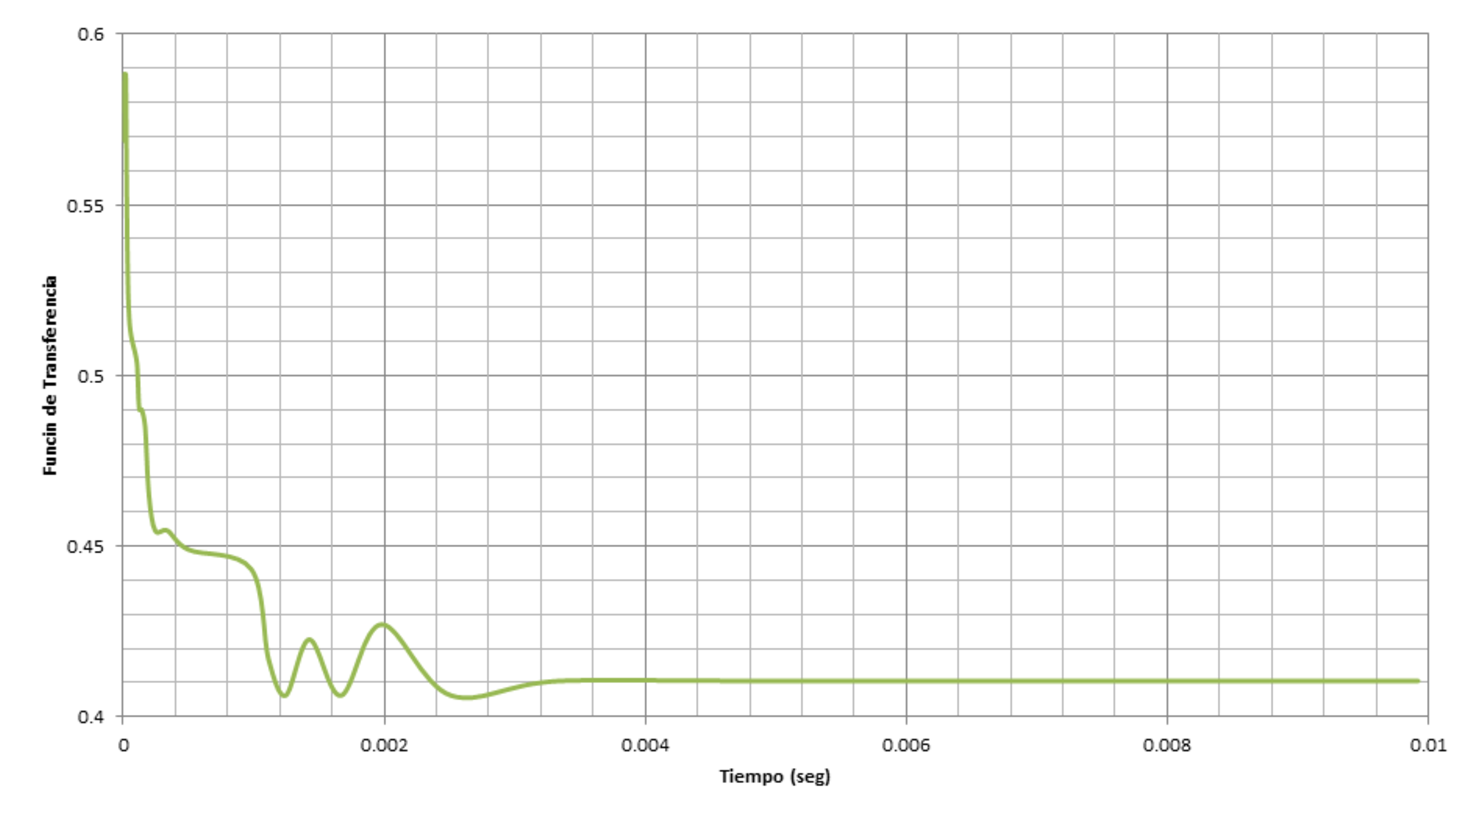
\includegraphics[width=1.00\textwidth]{ResReaFunL.eps}
	\caption{Funci\'on de Transferencia Real para el inductor}
	\label{cir:16}
\end{figure}

\begin{figure}[h]
	\centering
		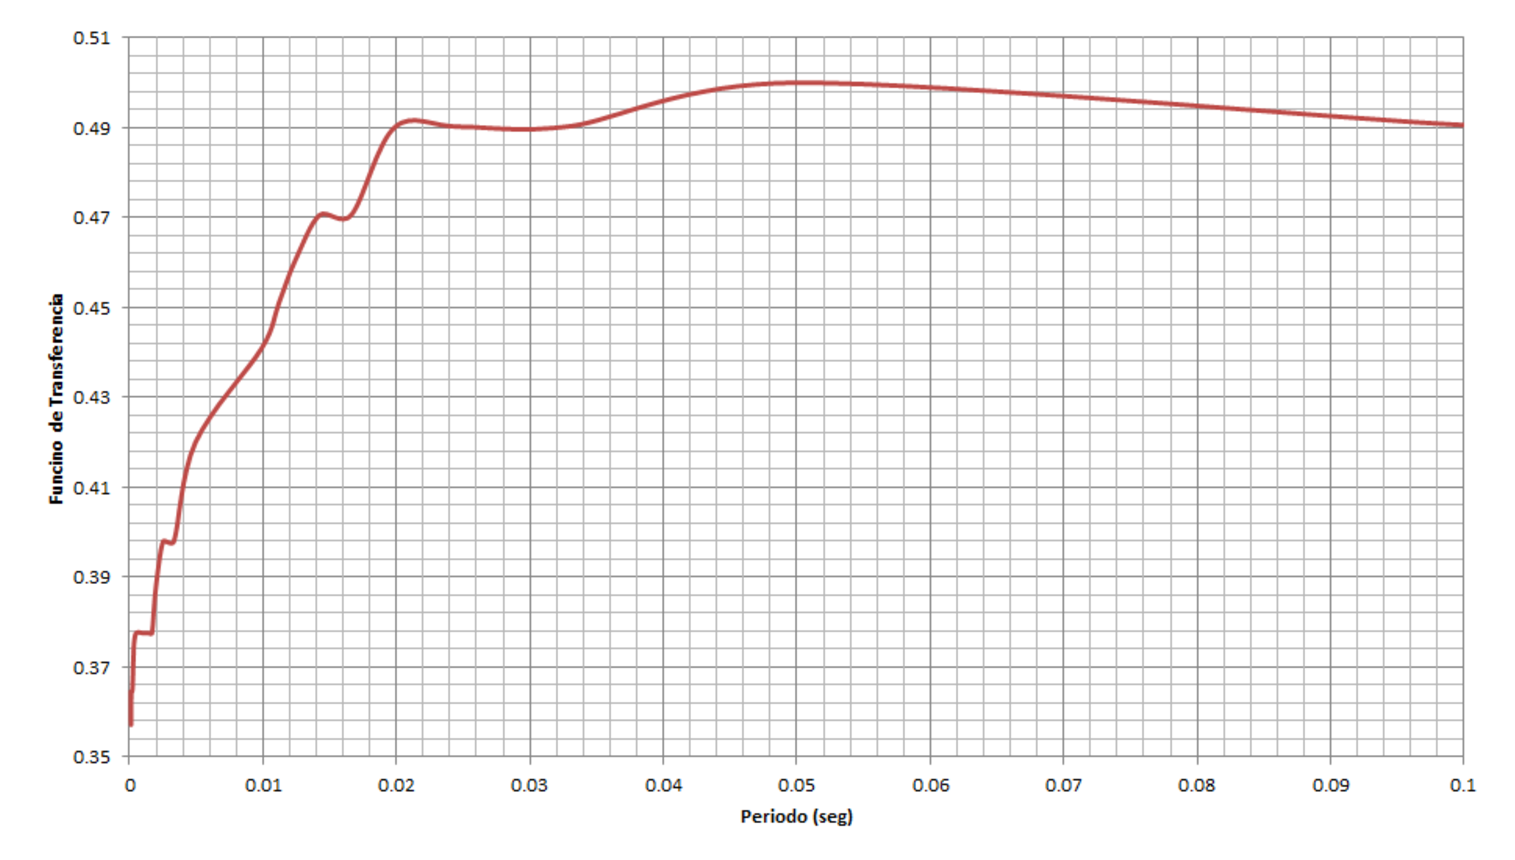
\includegraphics[width=1.00\textwidth]{ResReaFunC.eps}
	\caption{Funci\'on de Transferencia real para el capacitor}
	\label{cir:17}
\end{figure}

	\section{Tau}

Para encontrar $\tau$ de manera t\'eorica solo necesitamos analizar la forma est\'andar de la funci\'on de transferencia del circuito, si recordamos del reporte anterior, el termino $a$ de esta forma es el valor inverso de $\tau$, as\'i que viendo las formulas \ref{ecu:5} y \ref{ecu:9}, podemos deducir que los valores para los $\tau$ del capacitor y del inductor est\'an dados por las formulas \ref{ecu:10} y \ref{ecu:11} respectivamente.

	\begin{equation}
		\centering
		\tau = \frac{L_{1}(R_{1}+R_{3})}{R_{1}R_{2}+R_{1}R_{3}+R_{2}R_{3}}
		\label{ecu:10}
	\end{equation}

	\begin{equation}
		\centering
		\tau = \frac{C_{1}(R_{1}R_{2}+R_{1}R_{3}+R_{2}R_{3})}{R_{1}+R_{3}}
		\label{ecu:11}
	\end{equation}

Y sustituyendo los valores que utilizamos en para esta practica tenemos valores te\'oricos de $\tau$ igual a $28.33 \mu s$ para el capacitor y a $1.5 ms$ para el inductor.

	\section{Discusi\'on}

Como podemos ver, a lo largo del reporte, las formas de onda obtenidas del circuito real contrapuestas contra las obtenidas a trav\'es del modelado matem\'atico y simulaci\'on, son, de manera general, similares, obviamente existen factores externos, de tipo ''compensable'', como lo pueden ser las tolerancias de $+/- 5\% $ en los valores reales de las resistencias y del $10$ al $20 \%$ en el caso de los capacitores, las cuales en caso de ser un circuito en el que queramos tener los valores precisos podr\'iamos intentar compensar con mas resistencias o capacitores conectados en serie o paralelo; sin embargo tambi\'en existen factores no compensables como capacitancias, inductancias y resistencias paracitas, dadas por cables, y simplemente por los mismos componentes del circuito, estas no son compensables ni siquiera medibles en algunos casos, ademas de otras como temperatura, que si son medibles, pero no controlables.\\ Por lo cual, conociendo, por ende, que las simulaciones son aproximaciones te\'oricas para la respuesta de un circuito ideal, podemos concluir que lo obtenido en la parte f\'isica es aceptable, ya que si bien las formas de onda no son tan est\'eticas como en las predicciones que hicimos, estas tienen una respuesta similar a lo que esperamos.
\chapter{Conclusiones}
Concluyendo con esto que para un sistema, realizar un modelado matem\'atico o simulaci\'on es bastante \'util en el sentido de que tendremos una aproximaci\'on previa de que es lo que esperamos ver, teniendo con esto la posibilidad de analizar si realmente tendr\'a la respuesta que deseamos obtener o si sera \'util en la aplicaci\'on que intentamos darle, de tal manera que sera mas simple para nosotros comprobar si su funcionamiento es optimo, malo o muy deficiente, y que podemos hacer para arreglarlo o mejorarlo.

\end{document}



